\documentclass[twoside]{book}

% Packages required by doxygen
\usepackage{calc}
\usepackage{doxygen}
\usepackage{graphicx}
\usepackage[utf8]{inputenc}
\usepackage{makeidx}
\usepackage{multicol}
\usepackage{multirow}
\usepackage{textcomp}
\usepackage[table]{xcolor}

% Font selection
\usepackage[T1]{fontenc}
\usepackage{mathptmx}
\usepackage[scaled=.90]{helvet}
\usepackage{courier}
\usepackage{amssymb}
\usepackage{sectsty}
\renewcommand{\familydefault}{\sfdefault}
\allsectionsfont{%
  \fontseries{bc}\selectfont%
  \color{darkgray}%
}
\renewcommand{\DoxyLabelFont}{%
  \fontseries{bc}\selectfont%
  \color{darkgray}%
}

% Page & text layout
\usepackage{geometry}
\geometry{%
  a4paper,%
  top=2.5cm,%
  bottom=2.5cm,%
  left=2.5cm,%
  right=2.5cm%
}
\tolerance=750
\hfuzz=15pt
\hbadness=750
\setlength{\emergencystretch}{15pt}
\setlength{\parindent}{0cm}
\setlength{\parskip}{0.2cm}
\makeatletter
\renewcommand{\paragraph}{%
  \@startsection{paragraph}{4}{0ex}{-1.0ex}{1.0ex}{%
    \normalfont\normalsize\bfseries\SS@parafont%
  }%
}
\renewcommand{\subparagraph}{%
  \@startsection{subparagraph}{5}{0ex}{-1.0ex}{1.0ex}{%
    \normalfont\normalsize\bfseries\SS@subparafont%
  }%
}
\makeatother

% Headers & footers
\usepackage{fancyhdr}
\pagestyle{fancyplain}
\fancyhead[LE]{\fancyplain{}{\bfseries\thepage}}
\fancyhead[CE]{\fancyplain{}{}}
\fancyhead[RE]{\fancyplain{}{\bfseries\leftmark}}
\fancyhead[LO]{\fancyplain{}{\bfseries\rightmark}}
\fancyhead[CO]{\fancyplain{}{}}
\fancyhead[RO]{\fancyplain{}{\bfseries\thepage}}
\fancyfoot[LE]{\fancyplain{}{}}
\fancyfoot[CE]{\fancyplain{}{}}
\fancyfoot[RE]{\fancyplain{}{\bfseries\scriptsize Generated on Wed May 9 2018 09\-:19\-:12 for My Project by Doxygen }}
\fancyfoot[LO]{\fancyplain{}{\bfseries\scriptsize Generated on Wed May 9 2018 09\-:19\-:12 for My Project by Doxygen }}
\fancyfoot[CO]{\fancyplain{}{}}
\fancyfoot[RO]{\fancyplain{}{}}
\renewcommand{\footrulewidth}{0.4pt}
\renewcommand{\chaptermark}[1]{%
  \markboth{#1}{}%
}
\renewcommand{\sectionmark}[1]{%
  \markright{\thesection\ #1}%
}

% Indices & bibliography
\usepackage{natbib}
\usepackage[titles]{tocloft}
\setcounter{tocdepth}{3}
\setcounter{secnumdepth}{5}
\makeindex

% Hyperlinks (required, but should be loaded last)
\usepackage{ifpdf}
\ifpdf
  \usepackage[pdftex,pagebackref=true]{hyperref}
\else
  \usepackage[ps2pdf,pagebackref=true]{hyperref}
\fi
\hypersetup{%
  colorlinks=true,%
  linkcolor=blue,%
  citecolor=blue,%
  unicode%
}

% Custom commands
\newcommand{\clearemptydoublepage}{%
  \newpage{\pagestyle{empty}\cleardoublepage}%
}


%===== C O N T E N T S =====

\begin{document}

% Titlepage & ToC
\hypersetup{pageanchor=false}
\pagenumbering{roman}
\begin{titlepage}
\vspace*{7cm}
\begin{center}%
{\Large My Project }\\
\vspace*{1cm}
{\large Generated by Doxygen 1.8.5}\\
\vspace*{0.5cm}
{\small Wed May 9 2018 09:19:12}\\
\end{center}
\end{titlepage}
\clearemptydoublepage
\tableofcontents
\clearemptydoublepage
\pagenumbering{arabic}
\hypersetup{pageanchor=true}

%--- Begin generated contents ---
\chapter{Hierarchical Index}
\section{Class Hierarchy}
This inheritance list is sorted roughly, but not completely, alphabetically\-:\begin{DoxyCompactList}
\item \contentsline{section}{Dvector}{\pageref{classDvector}}{}
\item \contentsline{section}{Generique\-Vector}{\pageref{classGeneriqueVector}}{}
\item \contentsline{section}{Gerstner\-Wave}{\pageref{classGerstnerWave}}{}
\item \contentsline{section}{Height}{\pageref{classHeight}}{}
\item \contentsline{section}{Ocean}{\pageref{classOcean}}{}
\item \contentsline{section}{Wave\-Model}{\pageref{classWaveModel}}{}
\begin{DoxyCompactList}
\item \contentsline{section}{Gerstner\-Wave\-Model}{\pageref{classGerstnerWaveModel}}{}
\item \contentsline{section}{Philips\-Wave\-Model}{\pageref{classPhilipsWaveModel}}{}
\end{DoxyCompactList}
\end{DoxyCompactList}

\chapter{Class Index}
\section{Class List}
Here are the classes, structs, unions and interfaces with brief descriptions\-:\begin{DoxyCompactList}
\item\contentsline{section}{\hyperlink{classDvector}{Dvector} }{\pageref{classDvector}}{}
\item\contentsline{section}{\hyperlink{classGeneriqueVector}{Generique\-Vector} }{\pageref{classGeneriqueVector}}{}
\item\contentsline{section}{\hyperlink{classGerstnerWave}{Gerstner\-Wave} }{\pageref{classGerstnerWave}}{}
\item\contentsline{section}{\hyperlink{classGerstnerWaveModel}{Gerstner\-Wave\-Model} }{\pageref{classGerstnerWaveModel}}{}
\item\contentsline{section}{\hyperlink{classHeight}{Height} }{\pageref{classHeight}}{}
\item\contentsline{section}{\hyperlink{classOcean}{Ocean} }{\pageref{classOcean}}{}
\item\contentsline{section}{\hyperlink{classPhilipsWaveModel}{Philips\-Wave\-Model} }{\pageref{classPhilipsWaveModel}}{}
\item\contentsline{section}{\hyperlink{classWaveModel}{Wave\-Model} }{\pageref{classWaveModel}}{}
\end{DoxyCompactList}

\chapter{File Index}
\section{File List}
Here is a list of all documented files with brief descriptions\-:\begin{DoxyCompactList}
\item\contentsline{section}{\hyperlink{Dvector_8h}{Dvector.\-h} \\*Mise en place des vecteurs }{\pageref{Dvector_8h}}{}
\item\contentsline{section}{\hyperlink{GeneriqueVector_8h}{Generique\-Vector.\-h} \\*Mise en place de vecteurs complex }{\pageref{GeneriqueVector_8h}}{}
\item\contentsline{section}{\hyperlink{GerstnerWave_8h}{Gerstner\-Wave.\-h} \\*Mise en place des vecteurs avec la hauteur Gestern }{\pageref{GerstnerWave_8h}}{}
\item\contentsline{section}{\hyperlink{GerstnerWaveModel_8h}{Gerstner\-Wave\-Model.\-h} \\*Mise en place d'un vecteur de \hyperlink{classGerstnerWave}{Gerstner\-Wave} }{\pageref{GerstnerWaveModel_8h}}{}
\item\contentsline{section}{\hyperlink{Height_8cpp}{Height.\-cpp} \\*Mise en place de la hauteur }{\pageref{Height_8cpp}}{}
\item\contentsline{section}{\hyperlink{Height_8h}{Height.\-h} \\*Mise en place d'un vecteur de \hyperlink{classGerstnerWave}{Gerstner\-Wave} }{\pageref{Height_8h}}{}
\item\contentsline{section}{\hyperlink{main_8cpp}{main.\-cpp} \\*Programme test }{\pageref{main_8cpp}}{}
\item\contentsline{section}{\hyperlink{Ocean_8cpp}{Ocean.\-cpp} \\*Mise en place de l'ocean de vectur }{\pageref{Ocean_8cpp}}{}
\item\contentsline{section}{\hyperlink{Ocean_8h}{Ocean.\-h} \\*Mise en place de l'ocean de vectur }{\pageref{Ocean_8h}}{}
\item\contentsline{section}{\hyperlink{PhilipsWaveModel_8cpp}{Philips\-Wave\-Model.\-cpp} \\*Mise en place de vecteurs de philips }{\pageref{PhilipsWaveModel_8cpp}}{}
\item\contentsline{section}{\hyperlink{PhilipsWaveModel_8h}{Philips\-Wave\-Model.\-h} \\*Mise en place de vecteurs de philips }{\pageref{PhilipsWaveModel_8h}}{}
\item\contentsline{section}{\hyperlink{WaveModel_8cpp}{Wave\-Model.\-cpp} \\*Mise en place de la classe Wave model qui permet de créer la classe philips et gerstern }{\pageref{WaveModel_8cpp}}{}
\item\contentsline{section}{\hyperlink{WaveModel_8h}{Wave\-Model.\-h} \\*Mise en place de la classe Wave model qui permet de créer la classe philips et gerstern }{\pageref{WaveModel_8h}}{}
\end{DoxyCompactList}

\chapter{Class Documentation}
\hypertarget{classDvector}{\section{Dvector Class Reference}
\label{classDvector}\index{Dvector@{Dvector}}
}
\subsection*{Public Member Functions}
\begin{DoxyCompactItemize}
\item 
\hypertarget{classDvector_adf0f620df0feef3311f7d198e649a298}{\hyperlink{classDvector_adf0f620df0feef3311f7d198e649a298}{Dvector} ()}\label{classDvector_adf0f620df0feef3311f7d198e649a298}

\begin{DoxyCompactList}\small\item\em Constructeur. \end{DoxyCompactList}\item 
\hyperlink{classDvector_a613d5e3f0102d46f16d86650d48d9e43}{Dvector} (int longueur, int valeur)
\begin{DoxyCompactList}\small\item\em Constructeur. \end{DoxyCompactList}\item 
\hyperlink{classDvector_a42eb49f338cbf649e4360035c72f9fe2}{Dvector} (int longueur)
\begin{DoxyCompactList}\small\item\em Constructeur. \end{DoxyCompactList}\item 
\hyperlink{classDvector_acfdd0c5c022184d9a0163a3cb8dc3730}{Dvector} (\hyperlink{classDvector}{Dvector} const \&autre)
\begin{DoxyCompactList}\small\item\em Constructeur. \end{DoxyCompactList}\item 
\hyperlink{classDvector_a2f2c20eb463fe2fd695493b5d6871244}{Dvector} (std\-::string fichier)
\begin{DoxyCompactList}\small\item\em Permet d'écrire dans un dvecteur dans un fichier. \end{DoxyCompactList}\item 
\hypertarget{classDvector_a3156d0776c5da1a15685970200ec6b96}{\hyperlink{classDvector_a3156d0776c5da1a15685970200ec6b96}{$\sim$\-Dvector} ()}\label{classDvector_a3156d0776c5da1a15685970200ec6b96}

\begin{DoxyCompactList}\small\item\em Destructeur. \end{DoxyCompactList}\item 
void \hyperlink{classDvector_af66e4bdf60171463c01eea1039eecdb1}{display} (std\-::ostream \&str)
\begin{DoxyCompactList}\small\item\em Permet de sortir le \hyperlink{classDvector}{Dvector}. \end{DoxyCompactList}\item 
\hypertarget{classDvector_af92b914997c31751ca7f805f63e0d543}{int \hyperlink{classDvector_af92b914997c31751ca7f805f63e0d543}{size} () const }\label{classDvector_af92b914997c31751ca7f805f63e0d543}

\begin{DoxyCompactList}\small\item\em Permet d'accéder à la longueur d'un vecteur. \end{DoxyCompactList}\item 
\hypertarget{classDvector_a6fecdca0fbad7f928403597e322234b1}{void \hyperlink{classDvector_a6fecdca0fbad7f928403597e322234b1}{fill\-Randomly} ()}\label{classDvector_a6fecdca0fbad7f928403597e322234b1}

\begin{DoxyCompactList}\small\item\em Permet de remplir le vecteur de manière random. \end{DoxyCompactList}\item 
double \& \hyperlink{classDvector_a64778b07b2a7b3de33b3df47df658da9}{operator()} (int i) const 
\begin{DoxyCompactList}\small\item\em Operator () \end{DoxyCompactList}\item 
\hyperlink{classDvector}{Dvector} \& \hyperlink{classDvector_a7d450c46faf4b75de106393ae5e63822}{operator=} (const \hyperlink{classDvector}{Dvector} \&v)
\begin{DoxyCompactList}\small\item\em Operator =. \end{DoxyCompactList}\item 
\hyperlink{classDvector}{Dvector} \& \hyperlink{classDvector_ab685d2a323d7d574e746fe4020e313f9}{operator+=} (const \hyperlink{classDvector}{Dvector} \&v)
\begin{DoxyCompactList}\small\item\em Operator +=. \end{DoxyCompactList}\item 
\hyperlink{classDvector}{Dvector} \& \hyperlink{classDvector_ae6715a7bddbb865336d2ff13777721fd}{operator+=} (const double \&c)
\begin{DoxyCompactList}\small\item\em Operator +=. \end{DoxyCompactList}\item 
\hyperlink{classDvector}{Dvector} \& \hyperlink{classDvector_a65bae8452b5a6646f9502f72264aa481}{operator-\/=} (const \hyperlink{classDvector}{Dvector} \&v)
\begin{DoxyCompactList}\small\item\em Operator -\/=. \end{DoxyCompactList}\item 
\hyperlink{classDvector}{Dvector} \& \hyperlink{classDvector_aeb48276f329b6a856e64994acf0c854b}{operator-\/=} (const double \&c)
\begin{DoxyCompactList}\small\item\em Operator -\/=. \end{DoxyCompactList}\item 
\hyperlink{classDvector}{Dvector} \& \hyperlink{classDvector_a0f7f02faaa3c717594380a3dfc034ca8}{operator$\ast$=} (const \hyperlink{classDvector}{Dvector} \&v)
\begin{DoxyCompactList}\small\item\em Operator $\ast$=. \end{DoxyCompactList}\item 
\hyperlink{classDvector}{Dvector} \& \hyperlink{classDvector_a0b19a08b86a8727f40d00dace8ace639}{operator$\ast$=} (const double \&c)
\begin{DoxyCompactList}\small\item\em Operator $\ast$=. \end{DoxyCompactList}\item 
\hyperlink{classDvector}{Dvector} \& \hyperlink{classDvector_a7698c539c6c001639df1a01ea62e0d85}{operator/=} (const \hyperlink{classDvector}{Dvector} \&v)
\begin{DoxyCompactList}\small\item\em Operator /=. \end{DoxyCompactList}\item 
\hyperlink{classDvector}{Dvector} \& \hyperlink{classDvector_ac4c5f6c7fb7b4f34f080b3c8c77b0943}{operator/=} (const double \&c)
\begin{DoxyCompactList}\small\item\em Operator /=. \end{DoxyCompactList}\item 
bool \hyperlink{classDvector_ad5e212597ae0d0bcbb0bf6678b9b4aa9}{operator==} (const \hyperlink{classDvector}{Dvector} \&v)
\begin{DoxyCompactList}\small\item\em Operator ==. \end{DoxyCompactList}\item 
void \hyperlink{classDvector_a774377bf2c62ca9d51fcf198a7c82839}{resize} (const int \&taille, const double \&c)
\begin{DoxyCompactList}\small\item\em Permet de redimensionner notre vecteur avec une constante. \end{DoxyCompactList}\item 
double \hyperlink{classDvector_a56e10051db695ea7f8aaf3079ea45472}{pdt\-\_\-scalaire} (\hyperlink{classDvector}{Dvector} w)
\begin{DoxyCompactList}\small\item\em permet de faire le produit scalaire de deux vecteurs \end{DoxyCompactList}\end{DoxyCompactItemize}


\subsection{Constructor \& Destructor Documentation}
\hypertarget{classDvector_a613d5e3f0102d46f16d86650d48d9e43}{\index{Dvector@{Dvector}!Dvector@{Dvector}}
\index{Dvector@{Dvector}!Dvector@{Dvector}}
\subsubsection[{Dvector}]{\setlength{\rightskip}{0pt plus 5cm}Dvector\-::\-Dvector (
\begin{DoxyParamCaption}
\item[{int}]{longueur, }
\item[{int}]{valeur}
\end{DoxyParamCaption}
)}}\label{classDvector_a613d5e3f0102d46f16d86650d48d9e43}


Constructeur. 


\begin{DoxyParams}{Parameters}
{\em longueur} & \-: longueur initiale du vecteur \\
\hline
{\em valeur} & \-: valeur initiale du vecteur \\
\hline
\end{DoxyParams}
\hypertarget{classDvector_a42eb49f338cbf649e4360035c72f9fe2}{\index{Dvector@{Dvector}!Dvector@{Dvector}}
\index{Dvector@{Dvector}!Dvector@{Dvector}}
\subsubsection[{Dvector}]{\setlength{\rightskip}{0pt plus 5cm}Dvector\-::\-Dvector (
\begin{DoxyParamCaption}
\item[{int}]{longueur}
\end{DoxyParamCaption}
)}}\label{classDvector_a42eb49f338cbf649e4360035c72f9fe2}


Constructeur. 


\begin{DoxyParams}{Parameters}
{\em longueur} & \-: longueur initiale du vecteur \\
\hline
\end{DoxyParams}
\hypertarget{classDvector_acfdd0c5c022184d9a0163a3cb8dc3730}{\index{Dvector@{Dvector}!Dvector@{Dvector}}
\index{Dvector@{Dvector}!Dvector@{Dvector}}
\subsubsection[{Dvector}]{\setlength{\rightskip}{0pt plus 5cm}Dvector\-::\-Dvector (
\begin{DoxyParamCaption}
\item[{{\bf Dvector} const \&}]{autre}
\end{DoxyParamCaption}
)}}\label{classDvector_acfdd0c5c022184d9a0163a3cb8dc3730}


Constructeur. 


\begin{DoxyParams}{Parameters}
{\em autre} & \-: Dvecteur initiale \\
\hline
\end{DoxyParams}
\hypertarget{classDvector_a2f2c20eb463fe2fd695493b5d6871244}{\index{Dvector@{Dvector}!Dvector@{Dvector}}
\index{Dvector@{Dvector}!Dvector@{Dvector}}
\subsubsection[{Dvector}]{\setlength{\rightskip}{0pt plus 5cm}Dvector\-::\-Dvector (
\begin{DoxyParamCaption}
\item[{std\-::string}]{fichier}
\end{DoxyParamCaption}
)}}\label{classDvector_a2f2c20eb463fe2fd695493b5d6871244}


Permet d'écrire dans un dvecteur dans un fichier. 


\begin{DoxyParams}{Parameters}
{\em fichier} & \-: fichier dans lequel on écrit \\
\hline
\end{DoxyParams}


\subsection{Member Function Documentation}
\hypertarget{classDvector_af66e4bdf60171463c01eea1039eecdb1}{\index{Dvector@{Dvector}!display@{display}}
\index{display@{display}!Dvector@{Dvector}}
\subsubsection[{display}]{\setlength{\rightskip}{0pt plus 5cm}void Dvector\-::display (
\begin{DoxyParamCaption}
\item[{std\-::ostream \&}]{str}
\end{DoxyParamCaption}
)}}\label{classDvector_af66e4bdf60171463c01eea1039eecdb1}


Permet de sortir le \hyperlink{classDvector}{Dvector}. 


\begin{DoxyParams}{Parameters}
{\em str} & \-: zone d'ecriture \\
\hline
\end{DoxyParams}
\hypertarget{classDvector_a64778b07b2a7b3de33b3df47df658da9}{\index{Dvector@{Dvector}!operator()@{operator()}}
\index{operator()@{operator()}!Dvector@{Dvector}}
\subsubsection[{operator()}]{\setlength{\rightskip}{0pt plus 5cm}double \& Dvector\-::operator() (
\begin{DoxyParamCaption}
\item[{int}]{i}
\end{DoxyParamCaption}
) const}}\label{classDvector_a64778b07b2a7b3de33b3df47df658da9}


Operator () 


\begin{DoxyParams}{Parameters}
{\em i,un} & entier qui ne doit pas etre plus grand que la taille du vecteur \\
\hline
\end{DoxyParams}
\hypertarget{classDvector_a0f7f02faaa3c717594380a3dfc034ca8}{\index{Dvector@{Dvector}!operator$\ast$=@{operator$\ast$=}}
\index{operator$\ast$=@{operator$\ast$=}!Dvector@{Dvector}}
\subsubsection[{operator$\ast$=}]{\setlength{\rightskip}{0pt plus 5cm}{\bf Dvector} \& Dvector\-::operator$\ast$= (
\begin{DoxyParamCaption}
\item[{const {\bf Dvector} \&}]{v}
\end{DoxyParamCaption}
)}}\label{classDvector_a0f7f02faaa3c717594380a3dfc034ca8}


Operator $\ast$=. 


\begin{DoxyParams}{Parameters}
{\em v} & \\
\hline
\end{DoxyParams}
\begin{DoxyReturn}{Returns}
\hyperlink{classDvector}{Dvector} 
\end{DoxyReturn}
\hypertarget{classDvector_a0b19a08b86a8727f40d00dace8ace639}{\index{Dvector@{Dvector}!operator$\ast$=@{operator$\ast$=}}
\index{operator$\ast$=@{operator$\ast$=}!Dvector@{Dvector}}
\subsubsection[{operator$\ast$=}]{\setlength{\rightskip}{0pt plus 5cm}{\bf Dvector} \& Dvector\-::operator$\ast$= (
\begin{DoxyParamCaption}
\item[{const double \&}]{c}
\end{DoxyParamCaption}
)}}\label{classDvector_a0b19a08b86a8727f40d00dace8ace639}


Operator $\ast$=. 


\begin{DoxyParams}{Parameters}
{\em c} & \\
\hline
\end{DoxyParams}
\begin{DoxyReturn}{Returns}
\hyperlink{classDvector}{Dvector} 
\end{DoxyReturn}
\hypertarget{classDvector_ab685d2a323d7d574e746fe4020e313f9}{\index{Dvector@{Dvector}!operator+=@{operator+=}}
\index{operator+=@{operator+=}!Dvector@{Dvector}}
\subsubsection[{operator+=}]{\setlength{\rightskip}{0pt plus 5cm}{\bf Dvector} \& Dvector\-::operator+= (
\begin{DoxyParamCaption}
\item[{const {\bf Dvector} \&}]{v}
\end{DoxyParamCaption}
)}}\label{classDvector_ab685d2a323d7d574e746fe4020e313f9}


Operator +=. 


\begin{DoxyParams}{Parameters}
{\em v} & \\
\hline
\end{DoxyParams}
\begin{DoxyReturn}{Returns}
\hyperlink{classDvector}{Dvector} 
\end{DoxyReturn}
\hypertarget{classDvector_ae6715a7bddbb865336d2ff13777721fd}{\index{Dvector@{Dvector}!operator+=@{operator+=}}
\index{operator+=@{operator+=}!Dvector@{Dvector}}
\subsubsection[{operator+=}]{\setlength{\rightskip}{0pt plus 5cm}{\bf Dvector} \& Dvector\-::operator+= (
\begin{DoxyParamCaption}
\item[{const double \&}]{c}
\end{DoxyParamCaption}
)}}\label{classDvector_ae6715a7bddbb865336d2ff13777721fd}


Operator +=. 


\begin{DoxyParams}{Parameters}
{\em c} & \\
\hline
\end{DoxyParams}
\begin{DoxyReturn}{Returns}
\hyperlink{classDvector}{Dvector} 
\end{DoxyReturn}
\hypertarget{classDvector_a65bae8452b5a6646f9502f72264aa481}{\index{Dvector@{Dvector}!operator-\/=@{operator-\/=}}
\index{operator-\/=@{operator-\/=}!Dvector@{Dvector}}
\subsubsection[{operator-\/=}]{\setlength{\rightskip}{0pt plus 5cm}{\bf Dvector} \& Dvector\-::operator-\/= (
\begin{DoxyParamCaption}
\item[{const {\bf Dvector} \&}]{v}
\end{DoxyParamCaption}
)}}\label{classDvector_a65bae8452b5a6646f9502f72264aa481}


Operator -\/=. 


\begin{DoxyParams}{Parameters}
{\em v} & \\
\hline
\end{DoxyParams}
\begin{DoxyReturn}{Returns}
\hyperlink{classDvector}{Dvector} 
\end{DoxyReturn}
\hypertarget{classDvector_aeb48276f329b6a856e64994acf0c854b}{\index{Dvector@{Dvector}!operator-\/=@{operator-\/=}}
\index{operator-\/=@{operator-\/=}!Dvector@{Dvector}}
\subsubsection[{operator-\/=}]{\setlength{\rightskip}{0pt plus 5cm}{\bf Dvector} \& Dvector\-::operator-\/= (
\begin{DoxyParamCaption}
\item[{const double \&}]{c}
\end{DoxyParamCaption}
)}}\label{classDvector_aeb48276f329b6a856e64994acf0c854b}


Operator -\/=. 


\begin{DoxyParams}{Parameters}
{\em c} & \\
\hline
\end{DoxyParams}
\begin{DoxyReturn}{Returns}
\hyperlink{classDvector}{Dvector} 
\end{DoxyReturn}
\hypertarget{classDvector_a7698c539c6c001639df1a01ea62e0d85}{\index{Dvector@{Dvector}!operator/=@{operator/=}}
\index{operator/=@{operator/=}!Dvector@{Dvector}}
\subsubsection[{operator/=}]{\setlength{\rightskip}{0pt plus 5cm}{\bf Dvector} \& Dvector\-::operator/= (
\begin{DoxyParamCaption}
\item[{const {\bf Dvector} \&}]{v}
\end{DoxyParamCaption}
)}}\label{classDvector_a7698c539c6c001639df1a01ea62e0d85}


Operator /=. 


\begin{DoxyParams}{Parameters}
{\em v} & \\
\hline
\end{DoxyParams}
\begin{DoxyReturn}{Returns}
\hyperlink{classDvector}{Dvector} 
\end{DoxyReturn}
\hypertarget{classDvector_ac4c5f6c7fb7b4f34f080b3c8c77b0943}{\index{Dvector@{Dvector}!operator/=@{operator/=}}
\index{operator/=@{operator/=}!Dvector@{Dvector}}
\subsubsection[{operator/=}]{\setlength{\rightskip}{0pt plus 5cm}{\bf Dvector} \& Dvector\-::operator/= (
\begin{DoxyParamCaption}
\item[{const double \&}]{c}
\end{DoxyParamCaption}
)}}\label{classDvector_ac4c5f6c7fb7b4f34f080b3c8c77b0943}


Operator /=. 


\begin{DoxyParams}{Parameters}
{\em c} & \\
\hline
\end{DoxyParams}
\begin{DoxyReturn}{Returns}
\hyperlink{classDvector}{Dvector} 
\end{DoxyReturn}
\hypertarget{classDvector_a7d450c46faf4b75de106393ae5e63822}{\index{Dvector@{Dvector}!operator=@{operator=}}
\index{operator=@{operator=}!Dvector@{Dvector}}
\subsubsection[{operator=}]{\setlength{\rightskip}{0pt plus 5cm}{\bf Dvector} \& Dvector\-::operator= (
\begin{DoxyParamCaption}
\item[{const {\bf Dvector} \&}]{v}
\end{DoxyParamCaption}
)}}\label{classDvector_a7d450c46faf4b75de106393ae5e63822}


Operator =. 


\begin{DoxyParams}{Parameters}
{\em v} & \\
\hline
\end{DoxyParams}
\begin{DoxyReturn}{Returns}
\hyperlink{classDvector}{Dvector} 
\end{DoxyReturn}
\hypertarget{classDvector_ad5e212597ae0d0bcbb0bf6678b9b4aa9}{\index{Dvector@{Dvector}!operator==@{operator==}}
\index{operator==@{operator==}!Dvector@{Dvector}}
\subsubsection[{operator==}]{\setlength{\rightskip}{0pt plus 5cm}bool Dvector\-::operator== (
\begin{DoxyParamCaption}
\item[{const {\bf Dvector} \&}]{v}
\end{DoxyParamCaption}
)}}\label{classDvector_ad5e212597ae0d0bcbb0bf6678b9b4aa9}


Operator ==. 


\begin{DoxyParams}{Parameters}
{\em v} & \\
\hline
\end{DoxyParams}
\begin{DoxyReturn}{Returns}
bool 
\end{DoxyReturn}
\hypertarget{classDvector_a56e10051db695ea7f8aaf3079ea45472}{\index{Dvector@{Dvector}!pdt\-\_\-scalaire@{pdt\-\_\-scalaire}}
\index{pdt\-\_\-scalaire@{pdt\-\_\-scalaire}!Dvector@{Dvector}}
\subsubsection[{pdt\-\_\-scalaire}]{\setlength{\rightskip}{0pt plus 5cm}double Dvector\-::pdt\-\_\-scalaire (
\begin{DoxyParamCaption}
\item[{{\bf Dvector}}]{w}
\end{DoxyParamCaption}
)}}\label{classDvector_a56e10051db695ea7f8aaf3079ea45472}


permet de faire le produit scalaire de deux vecteurs 


\begin{DoxyParams}{Parameters}
{\em w} & \\
\hline
\end{DoxyParams}
\begin{DoxyReturn}{Returns}
double 
\end{DoxyReturn}
\hypertarget{classDvector_a774377bf2c62ca9d51fcf198a7c82839}{\index{Dvector@{Dvector}!resize@{resize}}
\index{resize@{resize}!Dvector@{Dvector}}
\subsubsection[{resize}]{\setlength{\rightskip}{0pt plus 5cm}void Dvector\-::resize (
\begin{DoxyParamCaption}
\item[{const int \&}]{taille, }
\item[{const double \&}]{c}
\end{DoxyParamCaption}
)}}\label{classDvector_a774377bf2c62ca9d51fcf198a7c82839}


Permet de redimensionner notre vecteur avec une constante. 


\begin{DoxyParams}{Parameters}
{\em taille} & \-: taille du nouveau vecteur \\
\hline
{\em c} & \-: constante a ajouter à la fin du vecteur \\
\hline
\end{DoxyParams}


The documentation for this class was generated from the following files\-:\begin{DoxyCompactItemize}
\item 
\hyperlink{Dvector_8h}{Dvector.\-h}\item 
Dvector.\-cpp\end{DoxyCompactItemize}

\hypertarget{classGeneriqueVector}{\section{Generique\-Vector Class Reference}
\label{classGeneriqueVector}\index{Generique\-Vector@{Generique\-Vector}}
}
\subsection*{Public Member Functions}
\begin{DoxyCompactItemize}
\item 
\hypertarget{classGeneriqueVector_a4dd110ae197c2f68233266280baa83aa}{{\bfseries Generique\-Vector} (int longueur, complex$<$ double $>$ valeur)}\label{classGeneriqueVector_a4dd110ae197c2f68233266280baa83aa}

\item 
\hypertarget{classGeneriqueVector_a65a61d5fe5417c4f6f1b6c451e135b7d}{{\bfseries Generique\-Vector} (int longueur)}\label{classGeneriqueVector_a65a61d5fe5417c4f6f1b6c451e135b7d}

\item 
\hypertarget{classGeneriqueVector_ac29c1fdc8e327dbb67a65dfeca012662}{{\bfseries Generique\-Vector} (\hyperlink{classGeneriqueVector}{Generique\-Vector} const \&autre)}\label{classGeneriqueVector_ac29c1fdc8e327dbb67a65dfeca012662}

\item 
\hypertarget{classGeneriqueVector_a5997fb9313f0161e5e5800be7df7a30e}{{\bfseries Generique\-Vector} (std\-::string fichier)}\label{classGeneriqueVector_a5997fb9313f0161e5e5800be7df7a30e}

\item 
\hypertarget{classGeneriqueVector_aee3879b6808f286ae00a21d569a4b2bf}{void {\bfseries display} (std\-::ostream \&str)}\label{classGeneriqueVector_aee3879b6808f286ae00a21d569a4b2bf}

\item 
\hypertarget{classGeneriqueVector_abcc638ba83b96e2a00e214584c0ac89b}{int {\bfseries size} () const }\label{classGeneriqueVector_abcc638ba83b96e2a00e214584c0ac89b}

\item 
\hypertarget{classGeneriqueVector_afd76e7455f9f55d5f5feabcd7261cc6e}{void {\bfseries fill\-Randomly} ()}\label{classGeneriqueVector_afd76e7455f9f55d5f5feabcd7261cc6e}

\item 
\hypertarget{classGeneriqueVector_af022ad2aa4c21bf3d18eb1fdc1c4e9d0}{complex$<$ double $>$ \& {\bfseries operator()} (int i) const }\label{classGeneriqueVector_af022ad2aa4c21bf3d18eb1fdc1c4e9d0}

\item 
\hypertarget{classGeneriqueVector_aa8d4ceb0be072d03157e5dc6f6abe41a}{\hyperlink{classGeneriqueVector}{Generique\-Vector} \& {\bfseries operator=} (const \hyperlink{classGeneriqueVector}{Generique\-Vector} \&v)}\label{classGeneriqueVector_aa8d4ceb0be072d03157e5dc6f6abe41a}

\item 
\hypertarget{classGeneriqueVector_a95936d97447a2b48a0de9427bdac9f37}{\hyperlink{classGeneriqueVector}{Generique\-Vector} \& {\bfseries operator+=} (const \hyperlink{classGeneriqueVector}{Generique\-Vector} \&v)}\label{classGeneriqueVector_a95936d97447a2b48a0de9427bdac9f37}

\item 
\hypertarget{classGeneriqueVector_a234a95695be5917b9c43eef48eb4ad5c}{\hyperlink{classGeneriqueVector}{Generique\-Vector} \& {\bfseries operator+=} (const double \&c)}\label{classGeneriqueVector_a234a95695be5917b9c43eef48eb4ad5c}

\item 
\hypertarget{classGeneriqueVector_aac0f2eb0adc5ac56a8aeefcbc024153a}{\hyperlink{classGeneriqueVector}{Generique\-Vector} \& {\bfseries operator-\/=} (const \hyperlink{classGeneriqueVector}{Generique\-Vector} \&v)}\label{classGeneriqueVector_aac0f2eb0adc5ac56a8aeefcbc024153a}

\item 
\hypertarget{classGeneriqueVector_aff635eca8cf7204047ab8f7b4fe516a0}{\hyperlink{classGeneriqueVector}{Generique\-Vector} \& {\bfseries operator-\/=} (const double \&c)}\label{classGeneriqueVector_aff635eca8cf7204047ab8f7b4fe516a0}

\item 
\hypertarget{classGeneriqueVector_adca64b00e3d0b5192300b999e5bce4df}{\hyperlink{classGeneriqueVector}{Generique\-Vector} \& {\bfseries operator$\ast$=} (const \hyperlink{classGeneriqueVector}{Generique\-Vector} \&v)}\label{classGeneriqueVector_adca64b00e3d0b5192300b999e5bce4df}

\item 
\hypertarget{classGeneriqueVector_a838ad15de3547ee91fa788c8fcba4a19}{\hyperlink{classGeneriqueVector}{Generique\-Vector} \& {\bfseries operator$\ast$=} (const double \&c)}\label{classGeneriqueVector_a838ad15de3547ee91fa788c8fcba4a19}

\item 
\hypertarget{classGeneriqueVector_a452081487df5168019341e03b4793f47}{\hyperlink{classGeneriqueVector}{Generique\-Vector} \& {\bfseries operator/=} (const \hyperlink{classGeneriqueVector}{Generique\-Vector} \&v)}\label{classGeneriqueVector_a452081487df5168019341e03b4793f47}

\item 
\hypertarget{classGeneriqueVector_ae487b7474cb5799256088c62bfd2ff9a}{\hyperlink{classGeneriqueVector}{Generique\-Vector} \& {\bfseries operator/=} (const double \&c)}\label{classGeneriqueVector_ae487b7474cb5799256088c62bfd2ff9a}

\item 
\hypertarget{classGeneriqueVector_a2fcc04d45c1668fdc6a61dd7c121db35}{bool {\bfseries operator==} (const \hyperlink{classGeneriqueVector}{Generique\-Vector} \&v)}\label{classGeneriqueVector_a2fcc04d45c1668fdc6a61dd7c121db35}

\item 
\hypertarget{classGeneriqueVector_ae560f9529566eed565fa1974522e2066}{void {\bfseries resize} (const int \&taille, const double \&c)}\label{classGeneriqueVector_ae560f9529566eed565fa1974522e2066}

\item 
\hypertarget{classGeneriqueVector_a45bd3db3b6b0db240f8872f0fe9e4ca6}{complex$<$ double $>$ {\bfseries pdt\-\_\-scalaire} (\hyperlink{classGeneriqueVector}{Generique\-Vector} w)}\label{classGeneriqueVector_a45bd3db3b6b0db240f8872f0fe9e4ca6}

\item 
\hypertarget{classGeneriqueVector_a94ff66f0fdf963c8d216012b9f79b238}{\hyperlink{classGeneriqueVector}{Generique\-Vector} {\bfseries fft} ()}\label{classGeneriqueVector_a94ff66f0fdf963c8d216012b9f79b238}

\item 
\hypertarget{classGeneriqueVector_af4ec7d272fec68853cc09bc7cd31303b}{\hyperlink{classGeneriqueVector}{Generique\-Vector} {\bfseries conjugue} ()}\label{classGeneriqueVector_af4ec7d272fec68853cc09bc7cd31303b}

\item 
\hypertarget{classGeneriqueVector_a47ed9d0808cc22d028188f974109f91c}{\hyperlink{classGeneriqueVector}{Generique\-Vector} {\bfseries conjuguedivise} ()}\label{classGeneriqueVector_a47ed9d0808cc22d028188f974109f91c}

\item 
\hypertarget{classGeneriqueVector_a0937bdd38f7b8015ded3c009cee3682c}{\hyperlink{classGeneriqueVector}{Generique\-Vector} {\bfseries ifft} ()}\label{classGeneriqueVector_a0937bdd38f7b8015ded3c009cee3682c}

\end{DoxyCompactItemize}
\subsection*{Public Attributes}
\begin{DoxyCompactItemize}
\item 
\hypertarget{classGeneriqueVector_afa9d183baf347df4930c8a4ce77bbff5}{complex$<$ double $>$ $\ast$ {\bfseries tab}}\label{classGeneriqueVector_afa9d183baf347df4930c8a4ce77bbff5}

\end{DoxyCompactItemize}


The documentation for this class was generated from the following files\-:\begin{DoxyCompactItemize}
\item 
\hyperlink{GeneriqueVector_8h}{Generique\-Vector.\-h}\item 
Generique\-Vector.\-cpp\end{DoxyCompactItemize}

\hypertarget{classGerstnerWave}{\section{Gerstner\-Wave Class Reference}
\label{classGerstnerWave}\index{Gerstner\-Wave@{Gerstner\-Wave}}
}
\subsection*{Public Member Functions}
\begin{DoxyCompactItemize}
\item 
\hyperlink{classGerstnerWave_a0045d1db79193644ca35bee5792a1b27}{Gerstner\-Wave} (double ampl, double phas, \hyperlink{classDvector}{Dvector} dir, double freq)
\begin{DoxyCompactList}\small\item\em constructeur avec initialisation des paramètres \end{DoxyCompactList}\item 
\hyperlink{classGerstnerWave_a14bf3cb2ed7f00cb86317beed8a1b79a}{Gerstner\-Wave} (const \hyperlink{classGerstnerWave}{Gerstner\-Wave} \&g)
\begin{DoxyCompactList}\small\item\em constructeur par copie \end{DoxyCompactList}\item 
\hypertarget{classGerstnerWave_af3df02ad2ba5fa164c83e332eabadfea}{\hyperlink{classGerstnerWave_af3df02ad2ba5fa164c83e332eabadfea}{$\sim$\-Gerstner\-Wave} ()}\label{classGerstnerWave_af3df02ad2ba5fa164c83e332eabadfea}

\begin{DoxyCompactList}\small\item\em destructeur \end{DoxyCompactList}\item 
\hypertarget{classGerstnerWave_af7652183f345e8fa3830230765fd66dc}{double \hyperlink{classGerstnerWave_af7652183f345e8fa3830230765fd66dc}{get\-Amplitude} () const }\label{classGerstnerWave_af7652183f345e8fa3830230765fd66dc}

\begin{DoxyCompactList}\small\item\em accesseur pour l'amplitude \end{DoxyCompactList}\item 
\hypertarget{classGerstnerWave_a6e7d08e560ccc9713cb0f195779ddbf5}{double \hyperlink{classGerstnerWave_a6e7d08e560ccc9713cb0f195779ddbf5}{get\-Phase} () const }\label{classGerstnerWave_a6e7d08e560ccc9713cb0f195779ddbf5}

\begin{DoxyCompactList}\small\item\em accesseur pour la phase \end{DoxyCompactList}\item 
\hypertarget{classGerstnerWave_a0da29133a4909347e29a5689aa0a8608}{\hyperlink{classDvector}{Dvector} \hyperlink{classGerstnerWave_a0da29133a4909347e29a5689aa0a8608}{get\-Direction} () const }\label{classGerstnerWave_a0da29133a4909347e29a5689aa0a8608}

\begin{DoxyCompactList}\small\item\em accesseur pour la direction \end{DoxyCompactList}\item 
\hypertarget{classGerstnerWave_aba276c45f82541ae705e887fcd713b8c}{double \hyperlink{classGerstnerWave_aba276c45f82541ae705e887fcd713b8c}{get\-Frequence} () const }\label{classGerstnerWave_aba276c45f82541ae705e887fcd713b8c}

\begin{DoxyCompactList}\small\item\em accesseur pour la fréquence \end{DoxyCompactList}\item 
\hyperlink{classGerstnerWave}{Gerstner\-Wave} \& \hyperlink{classGerstnerWave_a8580f5ccd3801c4d97ba89f8e55bf4bd}{operator=} (const \hyperlink{classGerstnerWave}{Gerstner\-Wave} \&g)
\begin{DoxyCompactList}\small\item\em operateur = \end{DoxyCompactList}\item 
double \hyperlink{classGerstnerWave_a19861f5ff98d978c98faeedfaabd1bec}{operator()} (double x, double y, double t) const 
\begin{DoxyCompactList}\small\item\em operateur permettant d'acceder a la classe comme un foncteur \end{DoxyCompactList}\item 
double \hyperlink{classGerstnerWave_a286b95dabb3280f03fa6c0c130bd22a3}{operator()} (double x, double y, double t)
\begin{DoxyCompactList}\small\item\em operateur permettant d'acceder a la classe comme un foncteur \end{DoxyCompactList}\end{DoxyCompactItemize}
\subsection*{Protected Attributes}
\begin{DoxyCompactItemize}
\item 
double \hyperlink{classGerstnerWave_ad6b1092e468e0126830317a310579f43}{\-\_\-amplitude}
\item 
double \hyperlink{classGerstnerWave_aee8b26bf0fd7274b7a8483f318d6c950}{\-\_\-phase}
\item 
\hyperlink{classDvector}{Dvector} \hyperlink{classGerstnerWave_a0a4926740fe7e170e5a9ca2b76815583}{\-\_\-direction\-Onde}
\item 
double \hyperlink{classGerstnerWave_ab49814056dd4b3258f04a206f7a6e920}{\-\_\-frequence}
\end{DoxyCompactItemize}


\subsection{Constructor \& Destructor Documentation}
\hypertarget{classGerstnerWave_a0045d1db79193644ca35bee5792a1b27}{\index{Gerstner\-Wave@{Gerstner\-Wave}!Gerstner\-Wave@{Gerstner\-Wave}}
\index{Gerstner\-Wave@{Gerstner\-Wave}!GerstnerWave@{Gerstner\-Wave}}
\subsubsection[{Gerstner\-Wave}]{\setlength{\rightskip}{0pt plus 5cm}Gerstner\-Wave\-::\-Gerstner\-Wave (
\begin{DoxyParamCaption}
\item[{double}]{ampl, }
\item[{double}]{phas, }
\item[{{\bf Dvector}}]{dir, }
\item[{double}]{freq}
\end{DoxyParamCaption}
)}}\label{classGerstnerWave_a0045d1db79193644ca35bee5792a1b27}


constructeur avec initialisation des paramètres 


\begin{DoxyParams}{Parameters}
{\em ampl} & \-: amplitude initiale du vecteur \\
\hline
{\em phas} & \-: phase initiale du vecteur \\
\hline
{\em dir} & \-: vecteur initiale \\
\hline
{\em freq} & \-: frequence initiale \\
\hline
\end{DoxyParams}
\hypertarget{classGerstnerWave_a14bf3cb2ed7f00cb86317beed8a1b79a}{\index{Gerstner\-Wave@{Gerstner\-Wave}!Gerstner\-Wave@{Gerstner\-Wave}}
\index{Gerstner\-Wave@{Gerstner\-Wave}!GerstnerWave@{Gerstner\-Wave}}
\subsubsection[{Gerstner\-Wave}]{\setlength{\rightskip}{0pt plus 5cm}Gerstner\-Wave\-::\-Gerstner\-Wave (
\begin{DoxyParamCaption}
\item[{const {\bf Gerstner\-Wave} \&}]{g}
\end{DoxyParamCaption}
)}}\label{classGerstnerWave_a14bf3cb2ed7f00cb86317beed8a1b79a}


constructeur par copie 


\begin{DoxyParams}{Parameters}
{\em g} & \-: \hyperlink{classGerstnerWave}{Gerstner\-Wave} \\
\hline
\end{DoxyParams}


\subsection{Member Function Documentation}
\hypertarget{classGerstnerWave_a19861f5ff98d978c98faeedfaabd1bec}{\index{Gerstner\-Wave@{Gerstner\-Wave}!operator()@{operator()}}
\index{operator()@{operator()}!GerstnerWave@{Gerstner\-Wave}}
\subsubsection[{operator()}]{\setlength{\rightskip}{0pt plus 5cm}double Gerstner\-Wave\-::operator() (
\begin{DoxyParamCaption}
\item[{double}]{x, }
\item[{double}]{y, }
\item[{double}]{t}
\end{DoxyParamCaption}
) const}}\label{classGerstnerWave_a19861f5ff98d978c98faeedfaabd1bec}


operateur permettant d'acceder a la classe comme un foncteur 


\begin{DoxyParams}{Parameters}
{\em x,y,t} & \\
\hline
\end{DoxyParams}
\begin{DoxyReturn}{Returns}
double 
\end{DoxyReturn}
\hypertarget{classGerstnerWave_a286b95dabb3280f03fa6c0c130bd22a3}{\index{Gerstner\-Wave@{Gerstner\-Wave}!operator()@{operator()}}
\index{operator()@{operator()}!GerstnerWave@{Gerstner\-Wave}}
\subsubsection[{operator()}]{\setlength{\rightskip}{0pt plus 5cm}double Gerstner\-Wave\-::operator() (
\begin{DoxyParamCaption}
\item[{double}]{x, }
\item[{double}]{y, }
\item[{double}]{t}
\end{DoxyParamCaption}
)}}\label{classGerstnerWave_a286b95dabb3280f03fa6c0c130bd22a3}


operateur permettant d'acceder a la classe comme un foncteur 


\begin{DoxyParams}{Parameters}
{\em x,y,t} & \\
\hline
\end{DoxyParams}
\begin{DoxyReturn}{Returns}
double 
\end{DoxyReturn}
\hypertarget{classGerstnerWave_a8580f5ccd3801c4d97ba89f8e55bf4bd}{\index{Gerstner\-Wave@{Gerstner\-Wave}!operator=@{operator=}}
\index{operator=@{operator=}!GerstnerWave@{Gerstner\-Wave}}
\subsubsection[{operator=}]{\setlength{\rightskip}{0pt plus 5cm}{\bf Gerstner\-Wave} \& Gerstner\-Wave\-::operator= (
\begin{DoxyParamCaption}
\item[{const {\bf Gerstner\-Wave} \&}]{g}
\end{DoxyParamCaption}
)}}\label{classGerstnerWave_a8580f5ccd3801c4d97ba89f8e55bf4bd}


operateur = 


\begin{DoxyParams}{Parameters}
{\em g} & \\
\hline
\end{DoxyParams}
\begin{DoxyReturn}{Returns}
\hyperlink{classGerstnerWave}{Gerstner\-Wave} 
\end{DoxyReturn}


\subsection{Member Data Documentation}
\hypertarget{classGerstnerWave_ad6b1092e468e0126830317a310579f43}{\index{Gerstner\-Wave@{Gerstner\-Wave}!\-\_\-amplitude@{\-\_\-amplitude}}
\index{\-\_\-amplitude@{\-\_\-amplitude}!GerstnerWave@{Gerstner\-Wave}}
\subsubsection[{\-\_\-amplitude}]{\setlength{\rightskip}{0pt plus 5cm}double Gerstner\-Wave\-::\-\_\-amplitude\hspace{0.3cm}{\ttfamily [protected]}}}\label{classGerstnerWave_ad6b1092e468e0126830317a310579f43}
Amplitude \hypertarget{classGerstnerWave_a0a4926740fe7e170e5a9ca2b76815583}{\index{Gerstner\-Wave@{Gerstner\-Wave}!\-\_\-direction\-Onde@{\-\_\-direction\-Onde}}
\index{\-\_\-direction\-Onde@{\-\_\-direction\-Onde}!GerstnerWave@{Gerstner\-Wave}}
\subsubsection[{\-\_\-direction\-Onde}]{\setlength{\rightskip}{0pt plus 5cm}{\bf Dvector} Gerstner\-Wave\-::\-\_\-direction\-Onde\hspace{0.3cm}{\ttfamily [protected]}}}\label{classGerstnerWave_a0a4926740fe7e170e5a9ca2b76815583}
Direction onde \hypertarget{classGerstnerWave_ab49814056dd4b3258f04a206f7a6e920}{\index{Gerstner\-Wave@{Gerstner\-Wave}!\-\_\-frequence@{\-\_\-frequence}}
\index{\-\_\-frequence@{\-\_\-frequence}!GerstnerWave@{Gerstner\-Wave}}
\subsubsection[{\-\_\-frequence}]{\setlength{\rightskip}{0pt plus 5cm}double Gerstner\-Wave\-::\-\_\-frequence\hspace{0.3cm}{\ttfamily [protected]}}}\label{classGerstnerWave_ab49814056dd4b3258f04a206f7a6e920}
Frequence \hypertarget{classGerstnerWave_aee8b26bf0fd7274b7a8483f318d6c950}{\index{Gerstner\-Wave@{Gerstner\-Wave}!\-\_\-phase@{\-\_\-phase}}
\index{\-\_\-phase@{\-\_\-phase}!GerstnerWave@{Gerstner\-Wave}}
\subsubsection[{\-\_\-phase}]{\setlength{\rightskip}{0pt plus 5cm}double Gerstner\-Wave\-::\-\_\-phase\hspace{0.3cm}{\ttfamily [protected]}}}\label{classGerstnerWave_aee8b26bf0fd7274b7a8483f318d6c950}
Phase 

The documentation for this class was generated from the following files\-:\begin{DoxyCompactItemize}
\item 
\hyperlink{GerstnerWave_8h}{Gerstner\-Wave.\-h}\item 
Gerstner\-Wave.\-cpp\end{DoxyCompactItemize}

\hypertarget{classGerstnerWaveModel}{\section{Gerstner\-Wave\-Model Class Reference}
\label{classGerstnerWaveModel}\index{Gerstner\-Wave\-Model@{Gerstner\-Wave\-Model}}
}
Inheritance diagram for Gerstner\-Wave\-Model\-:\begin{figure}[H]
\begin{center}
\leavevmode
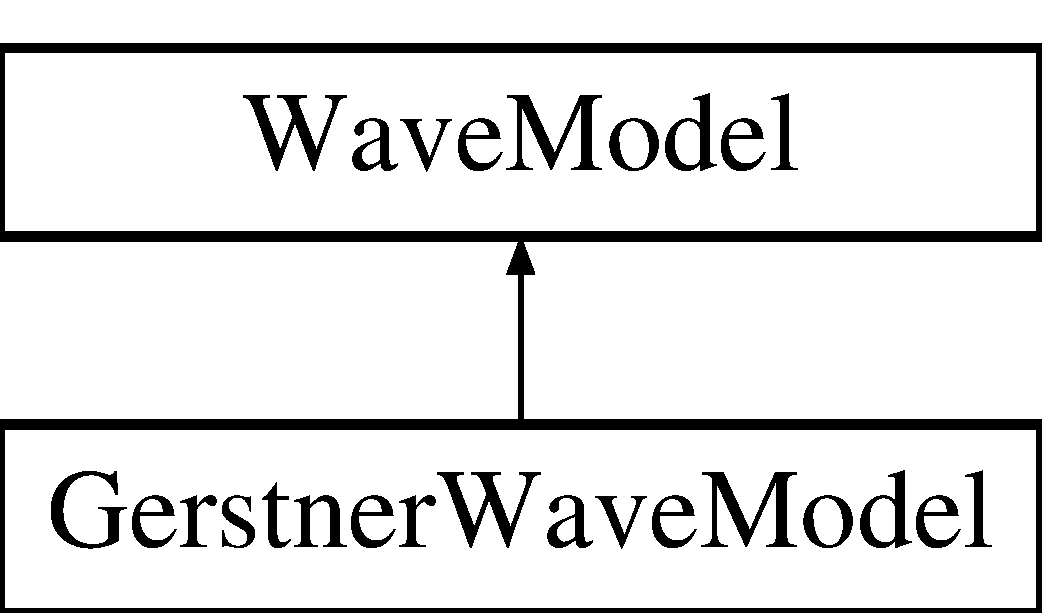
\includegraphics[height=2.000000cm]{classGerstnerWaveModel}
\end{center}
\end{figure}
\subsection*{Public Member Functions}
\begin{DoxyCompactItemize}
\item 
\hyperlink{classGerstnerWaveModel_a9b4ecbbc3abf2d9a9a66f95a28c5927d}{Gerstner\-Wave\-Model} (\hyperlink{classDvector}{Dvector} \hyperlink{classWaveModel_ab0ce1c49c362d60e89cef37e49cafb78}{\-\_\-direction}, double \hyperlink{classWaveModel_acbfbba2af6232fd3089615ab795a895e}{\-\_\-intensite})
\begin{DoxyCompactList}\small\item\em constructeur \end{DoxyCompactList}\item 
\hypertarget{classGerstnerWaveModel_ae14149452ec3a38f6e7b01eda5a3f034}{\hyperlink{classGerstnerWaveModel_ae14149452ec3a38f6e7b01eda5a3f034}{$\sim$\-Gerstner\-Wave\-Model} ()}\label{classGerstnerWaveModel_ae14149452ec3a38f6e7b01eda5a3f034}

\begin{DoxyCompactList}\small\item\em Destructeur. \end{DoxyCompactList}\item 
\hypertarget{classGerstnerWaveModel_aa5dbcf564026561f9e52f51ca1145e7e}{int {\bfseries get\-Nb\-\_\-ondes} ()}\label{classGerstnerWaveModel_aa5dbcf564026561f9e52f51ca1145e7e}

\item 
\hypertarget{classGerstnerWaveModel_a9409c817e45f7dd59d747da8135a61df}{std\-::vector$<$ \hyperlink{classDvector}{Dvector} $>$ {\bfseries get\-Ki} ()}\label{classGerstnerWaveModel_a9409c817e45f7dd59d747da8135a61df}

\item 
\hypertarget{classGerstnerWaveModel_a600e58d818a72b452c51566034bf37a0}{\hyperlink{classDvector}{Dvector} {\bfseries get\-Ai} ()}\label{classGerstnerWaveModel_a600e58d818a72b452c51566034bf37a0}

\item 
\hypertarget{classGerstnerWaveModel_a42ef93fd820ce54bb30151dd52b5acde}{\hyperlink{classDvector}{Dvector} {\bfseries get\-Wi} ()}\label{classGerstnerWaveModel_a42ef93fd820ce54bb30151dd52b5acde}

\item 
\hypertarget{classGerstnerWaveModel_a7fa71c326d76c5402341d53dd842b908}{\hyperlink{classDvector}{Dvector} {\bfseries get\-Phii} ()}\label{classGerstnerWaveModel_a7fa71c326d76c5402341d53dd842b908}

\item 
\hypertarget{classGerstnerWaveModel_a019545b256743495cdda97cfa723870b}{double \hyperlink{classGerstnerWaveModel_a019545b256743495cdda97cfa723870b}{operator()} (double x, double y, double t)}\label{classGerstnerWaveModel_a019545b256743495cdda97cfa723870b}

\begin{DoxyCompactList}\small\item\em operateur() \end{DoxyCompactList}\item 
\hypertarget{classGerstnerWaveModel_ab68423577985913106459a804549027c}{double \hyperlink{classGerstnerWaveModel_ab68423577985913106459a804549027c}{operator()} (double x, double y, double t) const }\label{classGerstnerWaveModel_ab68423577985913106459a804549027c}

\begin{DoxyCompactList}\small\item\em operateur() \end{DoxyCompactList}\end{DoxyCompactItemize}
\subsection*{Additional Inherited Members}


\subsection{Constructor \& Destructor Documentation}
\hypertarget{classGerstnerWaveModel_a9b4ecbbc3abf2d9a9a66f95a28c5927d}{\index{Gerstner\-Wave\-Model@{Gerstner\-Wave\-Model}!Gerstner\-Wave\-Model@{Gerstner\-Wave\-Model}}
\index{Gerstner\-Wave\-Model@{Gerstner\-Wave\-Model}!GerstnerWaveModel@{Gerstner\-Wave\-Model}}
\subsubsection[{Gerstner\-Wave\-Model}]{\setlength{\rightskip}{0pt plus 5cm}Gerstner\-Wave\-Model\-::\-Gerstner\-Wave\-Model (
\begin{DoxyParamCaption}
\item[{{\bf Dvector}}]{\-\_\-direction, }
\item[{double}]{\-\_\-intensite}
\end{DoxyParamCaption}
)}}\label{classGerstnerWaveModel_a9b4ecbbc3abf2d9a9a66f95a28c5927d}


constructeur 


\begin{DoxyParams}{Parameters}
{\em \-\_\-direction} & \-: Direction \\
\hline
{\em \-\_\-intensite} & \-: intensite \\
\hline
\end{DoxyParams}


The documentation for this class was generated from the following files\-:\begin{DoxyCompactItemize}
\item 
\hyperlink{GerstnerWaveModel_8h}{Gerstner\-Wave\-Model.\-h}\item 
Gerstner\-Wave\-Model.\-cpp\end{DoxyCompactItemize}

\hypertarget{classHeight}{\section{Height Class Reference}
\label{classHeight}\index{Height@{Height}}
}


{\ttfamily \#include $<$Height.\-h$>$}

\subsection*{Public Member Functions}
\begin{DoxyCompactItemize}
\item 
\hypertarget{classHeight_a7fecf5018a116f8234513b222bae6a2f}{\hyperlink{classHeight_a7fecf5018a116f8234513b222bae6a2f}{Height} ()}\label{classHeight_a7fecf5018a116f8234513b222bae6a2f}

\begin{DoxyCompactList}\small\item\em constructeur par defaut \end{DoxyCompactList}\item 
\hyperlink{classHeight_afef85fd5b8127c4bb4f27e05a4c869fe}{Height} (double l\-\_\-x, double l\-\_\-y, double n\-\_\-x, double n\-\_\-y)
\begin{DoxyCompactList}\small\item\em constructeur avec initialisation du tableau \end{DoxyCompactList}\item 
\hyperlink{classHeight_a2a357c8260db561016f559851ba3b831}{Height} (const \hyperlink{classHeight}{Height} \&h)
\begin{DoxyCompactList}\small\item\em constructeur par copie \end{DoxyCompactList}\item 
\hypertarget{classHeight_a93e56f89aa752196cc73ef5be717f386}{\hyperlink{classHeight_a93e56f89aa752196cc73ef5be717f386}{$\sim$\-Height} ()}\label{classHeight_a93e56f89aa752196cc73ef5be717f386}

\begin{DoxyCompactList}\small\item\em destructeur \end{DoxyCompactList}\item 
\hypertarget{classHeight_ac6ea0710f17f06938ea23aac943769b0}{\hyperlink{classDvector}{Dvector} \hyperlink{classHeight_ac6ea0710f17f06938ea23aac943769b0}{get\-Vector} () const }\label{classHeight_ac6ea0710f17f06938ea23aac943769b0}

\begin{DoxyCompactList}\small\item\em Accesseur au tableau des vecteurs. \end{DoxyCompactList}\item 
\hypertarget{classHeight_a483c8bc6157331b43069cff8149d88f1}{double \hyperlink{classHeight_a483c8bc6157331b43069cff8149d88f1}{get\-Lx} () const }\label{classHeight_a483c8bc6157331b43069cff8149d88f1}

\begin{DoxyCompactList}\small\item\em Accesseur a lx. \end{DoxyCompactList}\item 
\hypertarget{classHeight_aff1fa60b41395a3e55b87bb75082d50d}{double \hyperlink{classHeight_aff1fa60b41395a3e55b87bb75082d50d}{get\-Ly} () const }\label{classHeight_aff1fa60b41395a3e55b87bb75082d50d}

\begin{DoxyCompactList}\small\item\em Accesseur a ly. \end{DoxyCompactList}\item 
\hypertarget{classHeight_a29aae8ffba5cbf9262b0dbbf09ffe37d}{double \hyperlink{classHeight_a29aae8ffba5cbf9262b0dbbf09ffe37d}{get\-Nx} () const }\label{classHeight_a29aae8ffba5cbf9262b0dbbf09ffe37d}

\begin{DoxyCompactList}\small\item\em Accesseur a nx. \end{DoxyCompactList}\item 
\hypertarget{classHeight_acb97ec45437cf773f7d2256545c05f03}{double \hyperlink{classHeight_acb97ec45437cf773f7d2256545c05f03}{get\-Ny} () const }\label{classHeight_acb97ec45437cf773f7d2256545c05f03}

\begin{DoxyCompactList}\small\item\em Accesseur a ny. \end{DoxyCompactList}\item 
\hypertarget{classHeight_ac1f6dd58c6445abd25acec345eff1dad}{void {\bfseries set\-Lx} (double l\-\_\-x)}\label{classHeight_ac1f6dd58c6445abd25acec345eff1dad}

\item 
\hypertarget{classHeight_aba395aecd1274c86136e2b971bcde78a}{void {\bfseries set\-Ly} (double l\-\_\-y)}\label{classHeight_aba395aecd1274c86136e2b971bcde78a}

\item 
\hypertarget{classHeight_afa9d764aafd73d54a4758850c7818a41}{void {\bfseries set\-Nx} (double n\-\_\-x)}\label{classHeight_afa9d764aafd73d54a4758850c7818a41}

\item 
\hypertarget{classHeight_a6fb16d367a776466c8f889faa3b27cbf}{void {\bfseries set\-Ny} (double n\-\_\-y)}\label{classHeight_a6fb16d367a776466c8f889faa3b27cbf}

\item 
\hypertarget{classHeight_a644ca7635b73547aa0723ff1e9a97298}{void {\bfseries set\-Vector} (\hyperlink{classDvector}{Dvector} vect)}\label{classHeight_a644ca7635b73547aa0723ff1e9a97298}

\item 
double \& \hyperlink{classHeight_ade1c0807cbe1097b22436f8f0d857079}{operator()} (int off) const 
\begin{DoxyCompactList}\small\item\em operateur() \end{DoxyCompactList}\item 
\hyperlink{classHeight}{Height} \& \hyperlink{classHeight_a349ae0404a4c5e27616c8ca3ff25fa0d}{operator=} (const \hyperlink{classHeight}{Height} \&h)
\begin{DoxyCompactList}\small\item\em operateur d'affectation \end{DoxyCompactList}\end{DoxyCompactItemize}


\subsection{Detailed Description}
Classe qui contient l'ensemble des hauteurs calculées dans une boite carrée de taille physique (Lx, Ly) discretisee en (nx, ny) elements 

\subsection{Constructor \& Destructor Documentation}
\hypertarget{classHeight_afef85fd5b8127c4bb4f27e05a4c869fe}{\index{Height@{Height}!Height@{Height}}
\index{Height@{Height}!Height@{Height}}
\subsubsection[{Height}]{\setlength{\rightskip}{0pt plus 5cm}Height\-::\-Height (
\begin{DoxyParamCaption}
\item[{double}]{l\-\_\-x, }
\item[{double}]{l\-\_\-y, }
\item[{double}]{n\-\_\-x, }
\item[{double}]{n\-\_\-y}
\end{DoxyParamCaption}
)}}\label{classHeight_afef85fd5b8127c4bb4f27e05a4c869fe}


constructeur avec initialisation du tableau 


\begin{DoxyParams}{Parameters}
{\em l\-\_\-x,l\-\_\-y,n\-\_\-x,n\-\_\-y} & \\
\hline
\end{DoxyParams}
\hypertarget{classHeight_a2a357c8260db561016f559851ba3b831}{\index{Height@{Height}!Height@{Height}}
\index{Height@{Height}!Height@{Height}}
\subsubsection[{Height}]{\setlength{\rightskip}{0pt plus 5cm}Height\-::\-Height (
\begin{DoxyParamCaption}
\item[{const {\bf Height} \&}]{h}
\end{DoxyParamCaption}
)}}\label{classHeight_a2a357c8260db561016f559851ba3b831}


constructeur par copie 


\begin{DoxyParams}{Parameters}
{\em h} & \\
\hline
\end{DoxyParams}


\subsection{Member Function Documentation}
\hypertarget{classHeight_ade1c0807cbe1097b22436f8f0d857079}{\index{Height@{Height}!operator()@{operator()}}
\index{operator()@{operator()}!Height@{Height}}
\subsubsection[{operator()}]{\setlength{\rightskip}{0pt plus 5cm}double \& Height\-::operator() (
\begin{DoxyParamCaption}
\item[{int}]{off}
\end{DoxyParamCaption}
) const}}\label{classHeight_ade1c0807cbe1097b22436f8f0d857079}


operateur() 


\begin{DoxyParams}{Parameters}
{\em off} & \\
\hline
\end{DoxyParams}
\hypertarget{classHeight_a349ae0404a4c5e27616c8ca3ff25fa0d}{\index{Height@{Height}!operator=@{operator=}}
\index{operator=@{operator=}!Height@{Height}}
\subsubsection[{operator=}]{\setlength{\rightskip}{0pt plus 5cm}{\bf Height} \& Height\-::operator= (
\begin{DoxyParamCaption}
\item[{const {\bf Height} \&}]{h}
\end{DoxyParamCaption}
)}}\label{classHeight_a349ae0404a4c5e27616c8ca3ff25fa0d}


operateur d'affectation 


\begin{DoxyParams}{Parameters}
{\em h} & \\
\hline
\end{DoxyParams}


The documentation for this class was generated from the following files\-:\begin{DoxyCompactItemize}
\item 
\hyperlink{Height_8h}{Height.\-h}\item 
\hyperlink{Height_8cpp}{Height.\-cpp}\end{DoxyCompactItemize}

\hypertarget{classOcean}{\section{Ocean Class Reference}
\label{classOcean}\index{Ocean@{Ocean}}
}
\subsection*{Public Member Functions}
\begin{DoxyCompactItemize}
\item 
\hypertarget{classOcean_ae95ec123060d04d915786e179b5cb9d4}{\hyperlink{classOcean_ae95ec123060d04d915786e179b5cb9d4}{$\sim$\-Ocean} ()}\label{classOcean_ae95ec123060d04d915786e179b5cb9d4}

\begin{DoxyCompactList}\small\item\em destructeur \end{DoxyCompactList}\item 
\hyperlink{classOcean_ad22d62e38937baed49b9caa07389353e}{Ocean} (double lx, double ly, int nx, int ny, double t, \hyperlink{classWaveModel}{Wave\-Model} $\ast$model)
\begin{DoxyCompactList}\small\item\em constructeur \end{DoxyCompactList}\item 
\hyperlink{classHeight}{Height} \hyperlink{classOcean_aa21e615ed5fd15a78c7ccee3c91e2fe3}{get\-Hauteur} () const 
\item 
\hypertarget{classOcean_a4376d66f1d9616a48655d195ac442b12}{void {\bfseries set\-Vector\-Hauteur} (\hyperlink{classDvector}{Dvector} vecteur)}\label{classOcean_a4376d66f1d9616a48655d195ac442b12}

\item 
\hypertarget{classOcean_aff51c24de31612bfdd97ab64becc44f4}{void {\bfseries set\-Hauteur} (double haut)}\label{classOcean_aff51c24de31612bfdd97ab64becc44f4}

\item 
\hypertarget{classOcean_ac140ad8d9c78fbf179d83102b4ef4d06}{void \hyperlink{classOcean_ac140ad8d9c78fbf179d83102b4ef4d06}{compute} ()}\label{classOcean_ac140ad8d9c78fbf179d83102b4ef4d06}

\begin{DoxyCompactList}\small\item\em Permet d'accéder à la hauteur model. \end{DoxyCompactList}\item 
\hypertarget{classOcean_ad49f987b9a82294ea0a44ba7ffd63278}{void \hyperlink{classOcean_ad49f987b9a82294ea0a44ba7ffd63278}{gl\-\_\-vertices} (double h\-\_\-init)}\label{classOcean_ad49f987b9a82294ea0a44ba7ffd63278}

\begin{DoxyCompactList}\small\item\em permet de créer un vecteur de hauteurs \end{DoxyCompactList}\item 
\hypertarget{classOcean_a2c62a21b1e9d54ae18c912a85e9f520a}{void \hyperlink{classOcean_a2c62a21b1e9d54ae18c912a85e9f520a}{computeset} ()}\label{classOcean_a2c62a21b1e9d54ae18c912a85e9f520a}

\begin{DoxyCompactList}\small\item\em permet de set un model \end{DoxyCompactList}\end{DoxyCompactItemize}


\subsection{Constructor \& Destructor Documentation}
\hypertarget{classOcean_ad22d62e38937baed49b9caa07389353e}{\index{Ocean@{Ocean}!Ocean@{Ocean}}
\index{Ocean@{Ocean}!Ocean@{Ocean}}
\subsubsection[{Ocean}]{\setlength{\rightskip}{0pt plus 5cm}Ocean\-::\-Ocean (
\begin{DoxyParamCaption}
\item[{double}]{lx, }
\item[{double}]{ly, }
\item[{int}]{nx, }
\item[{int}]{ny, }
\item[{double}]{t, }
\item[{{\bf Wave\-Model} $\ast$}]{model}
\end{DoxyParamCaption}
)}}\label{classOcean_ad22d62e38937baed49b9caa07389353e}


constructeur 


\begin{DoxyParams}{Parameters}
{\em lx,ly,nx,ny,t,model} & \\
\hline
\end{DoxyParams}


\subsection{Member Function Documentation}
\hypertarget{classOcean_aa21e615ed5fd15a78c7ccee3c91e2fe3}{\index{Ocean@{Ocean}!get\-Hauteur@{get\-Hauteur}}
\index{get\-Hauteur@{get\-Hauteur}!Ocean@{Ocean}}
\subsubsection[{get\-Hauteur}]{\setlength{\rightskip}{0pt plus 5cm}{\bf Height} Ocean\-::get\-Hauteur (
\begin{DoxyParamCaption}
{}
\end{DoxyParamCaption}
) const\hspace{0.3cm}{\ttfamily [inline]}}}\label{classOcean_aa21e615ed5fd15a78c7ccee3c91e2fe3}
à la hauteur 

The documentation for this class was generated from the following files\-:\begin{DoxyCompactItemize}
\item 
\hyperlink{Ocean_8h}{Ocean.\-h}\item 
\hyperlink{Ocean_8cpp}{Ocean.\-cpp}\end{DoxyCompactItemize}

\hypertarget{classPhilipsWaveModel}{\section{Philips\-Wave\-Model Class Reference}
\label{classPhilipsWaveModel}\index{Philips\-Wave\-Model@{Philips\-Wave\-Model}}
}
Inheritance diagram for Philips\-Wave\-Model\-:\begin{figure}[H]
\begin{center}
\leavevmode
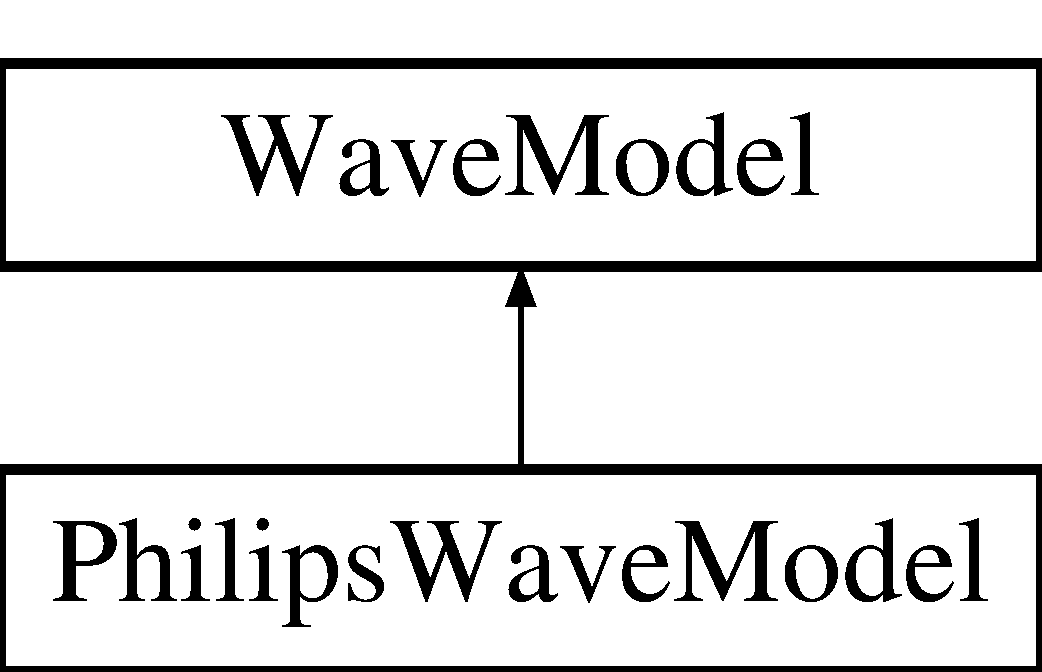
\includegraphics[height=2.000000cm]{classPhilipsWaveModel}
\end{center}
\end{figure}
\subsection*{Public Member Functions}
\begin{DoxyCompactItemize}
\item 
\hypertarget{classPhilipsWaveModel_a5fd60088cfeb35cdc529c4fadbaecf11}{\hyperlink{classPhilipsWaveModel_a5fd60088cfeb35cdc529c4fadbaecf11}{$\sim$\-Philips\-Wave\-Model} ()}\label{classPhilipsWaveModel_a5fd60088cfeb35cdc529c4fadbaecf11}

\begin{DoxyCompactList}\small\item\em destructeur \end{DoxyCompactList}\item 
\hyperlink{classPhilipsWaveModel_a9cb93d728be1a04bc0be2fcf5ce2f4e6}{Philips\-Wave\-Model} (\hyperlink{classDvector}{Dvector} vent\-\_\-direction, double intensite)
\begin{DoxyCompactList}\small\item\em constructeur \end{DoxyCompactList}\item 
\hypertarget{classPhilipsWaveModel_a2b6f3936d3294a056968a9ef37d051b0}{double \hyperlink{classPhilipsWaveModel_a2b6f3936d3294a056968a9ef37d051b0}{operator()} (double x, double y, double t)}\label{classPhilipsWaveModel_a2b6f3936d3294a056968a9ef37d051b0}

\begin{DoxyCompactList}\small\item\em operator (); \end{DoxyCompactList}\item 
\hypertarget{classPhilipsWaveModel_ac5d3959472111670ef05189a7bdeb379}{double \hyperlink{classPhilipsWaveModel_ac5d3959472111670ef05189a7bdeb379}{operator()} (double x, double y, double t) const }\label{classPhilipsWaveModel_ac5d3959472111670ef05189a7bdeb379}

\begin{DoxyCompactList}\small\item\em operateur() \end{DoxyCompactList}\item 
\hypertarget{classPhilipsWaveModel_a0c15316c6ebc65730f97b34d751faca8}{\hyperlink{classDvector}{Dvector} {\bfseries operator()} (double t)}\label{classPhilipsWaveModel_a0c15316c6ebc65730f97b34d751faca8}

\item 
double \hyperlink{classPhilipsWaveModel_aa61d74cb3a5495420eafac250b2961bb}{houle} (double kx, double ky)
\begin{DoxyCompactList}\small\item\em permet de calculer la houle \end{DoxyCompactList}\end{DoxyCompactItemize}
\subsection*{Additional Inherited Members}


\subsection{Constructor \& Destructor Documentation}
\hypertarget{classPhilipsWaveModel_a9cb93d728be1a04bc0be2fcf5ce2f4e6}{\index{Philips\-Wave\-Model@{Philips\-Wave\-Model}!Philips\-Wave\-Model@{Philips\-Wave\-Model}}
\index{Philips\-Wave\-Model@{Philips\-Wave\-Model}!PhilipsWaveModel@{Philips\-Wave\-Model}}
\subsubsection[{Philips\-Wave\-Model}]{\setlength{\rightskip}{0pt plus 5cm}Philips\-Wave\-Model\-::\-Philips\-Wave\-Model (
\begin{DoxyParamCaption}
\item[{{\bf Dvector}}]{vent\-\_\-direction, }
\item[{double}]{intensite}
\end{DoxyParamCaption}
)}}\label{classPhilipsWaveModel_a9cb93d728be1a04bc0be2fcf5ce2f4e6}


constructeur 


\begin{DoxyParams}{Parameters}
{\em direction} & du vent, intensité \\
\hline
\end{DoxyParams}


\subsection{Member Function Documentation}
\hypertarget{classPhilipsWaveModel_aa61d74cb3a5495420eafac250b2961bb}{\index{Philips\-Wave\-Model@{Philips\-Wave\-Model}!houle@{houle}}
\index{houle@{houle}!PhilipsWaveModel@{Philips\-Wave\-Model}}
\subsubsection[{houle}]{\setlength{\rightskip}{0pt plus 5cm}double Philips\-Wave\-Model\-::houle (
\begin{DoxyParamCaption}
\item[{double}]{kx, }
\item[{double}]{ky}
\end{DoxyParamCaption}
)}}\label{classPhilipsWaveModel_aa61d74cb3a5495420eafac250b2961bb}


permet de calculer la houle 


\begin{DoxyParams}{Parameters}
{\em kx,ky} & \\
\hline
\end{DoxyParams}


The documentation for this class was generated from the following files\-:\begin{DoxyCompactItemize}
\item 
\hyperlink{PhilipsWaveModel_8h}{Philips\-Wave\-Model.\-h}\item 
\hyperlink{PhilipsWaveModel_8cpp}{Philips\-Wave\-Model.\-cpp}\end{DoxyCompactItemize}

\hypertarget{classWaveModel}{\section{Wave\-Model Class Reference}
\label{classWaveModel}\index{Wave\-Model@{Wave\-Model}}
}
Inheritance diagram for Wave\-Model\-:\begin{figure}[H]
\begin{center}
\leavevmode
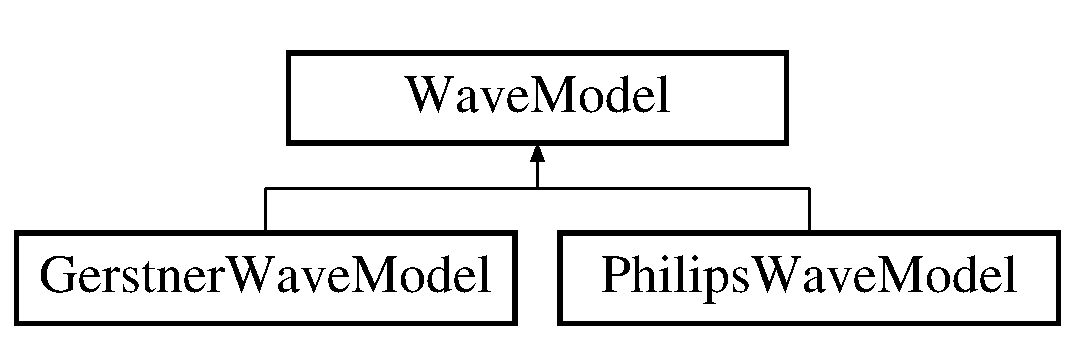
\includegraphics[height=2.000000cm]{classWaveModel}
\end{center}
\end{figure}
\subsection*{Public Member Functions}
\begin{DoxyCompactItemize}
\item 
\hypertarget{classWaveModel_a3bf52f16322370656b8711a68ce5d194}{\hyperlink{classWaveModel_a3bf52f16322370656b8711a68ce5d194}{Wave\-Model} ()}\label{classWaveModel_a3bf52f16322370656b8711a68ce5d194}

\begin{DoxyCompactList}\small\item\em constructeur par defaut \end{DoxyCompactList}\item 
\hypertarget{classWaveModel_afe136a278dbd88362d0b28220c70bcba}{\hyperlink{classWaveModel_afe136a278dbd88362d0b28220c70bcba}{Wave\-Model} (\hyperlink{classDvector}{Dvector} dir, \hyperlink{classDvector}{Dvector} align, double inte, double longu, double ajust)}\label{classWaveModel_afe136a278dbd88362d0b28220c70bcba}

\begin{DoxyCompactList}\small\item\em constructeur avec valeurs \end{DoxyCompactList}\item 
\hyperlink{classWaveModel_a15efb97c38955e3b5cacacf27b20e65b}{Wave\-Model} (const \hyperlink{classWaveModel}{Wave\-Model} \&w)
\begin{DoxyCompactList}\small\item\em constructeur par copie \end{DoxyCompactList}\item 
\hypertarget{classWaveModel_a83b17b2ec70b9ace55d5b3872f75dcce}{virtual \hyperlink{classWaveModel_a83b17b2ec70b9ace55d5b3872f75dcce}{$\sim$\-Wave\-Model} ()}\label{classWaveModel_a83b17b2ec70b9ace55d5b3872f75dcce}

\begin{DoxyCompactList}\small\item\em destructeur \end{DoxyCompactList}\item 
virtual \hyperlink{classWaveModel}{Wave\-Model} \& \hyperlink{classWaveModel_acbbb099975edc7b7ef03b23deb67bd68}{operator=} (const \hyperlink{classWaveModel}{Wave\-Model} \&w)
\begin{DoxyCompactList}\small\item\em operateur d'affectation = \end{DoxyCompactList}\item 
\hypertarget{classWaveModel_aaa56c92a70a69883a0d3c4da642f3d7b}{virtual \hyperlink{classDvector}{Dvector} \hyperlink{classWaveModel_aaa56c92a70a69883a0d3c4da642f3d7b}{get\-Direction} () const }\label{classWaveModel_aaa56c92a70a69883a0d3c4da642f3d7b}

\begin{DoxyCompactList}\small\item\em accesseur direction \end{DoxyCompactList}\item 
\hypertarget{classWaveModel_a2071bf319952d0a92b8724e930304261}{virtual \hyperlink{classDvector}{Dvector} \hyperlink{classWaveModel_a2071bf319952d0a92b8724e930304261}{get\-Alignement} () const }\label{classWaveModel_a2071bf319952d0a92b8724e930304261}

\begin{DoxyCompactList}\small\item\em accesseur alignement \end{DoxyCompactList}\item 
\hypertarget{classWaveModel_ae89da87502a9d4aed28897622a4388b7}{virtual double \hyperlink{classWaveModel_ae89da87502a9d4aed28897622a4388b7}{get\-Intensite} () const }\label{classWaveModel_ae89da87502a9d4aed28897622a4388b7}

\begin{DoxyCompactList}\small\item\em accesseur intensite \end{DoxyCompactList}\item 
\hypertarget{classWaveModel_a4fb84ba8f4904d1da2141faf787288c2}{virtual double \hyperlink{classWaveModel_a4fb84ba8f4904d1da2141faf787288c2}{get\-Longueur} () const }\label{classWaveModel_a4fb84ba8f4904d1da2141faf787288c2}

\begin{DoxyCompactList}\small\item\em accesseur longueur \end{DoxyCompactList}\item 
\hypertarget{classWaveModel_a511f75ab038ce7e25626dd8978d04705}{virtual double \hyperlink{classWaveModel_a511f75ab038ce7e25626dd8978d04705}{get\-Ajustement} () const }\label{classWaveModel_a511f75ab038ce7e25626dd8978d04705}

\begin{DoxyCompactList}\small\item\em accesseur ajustement \end{DoxyCompactList}\item 
\hypertarget{classWaveModel_a66612d80d52ef2619c7437f6ef26ac86}{virtual double \hyperlink{classWaveModel_a66612d80d52ef2619c7437f6ef26ac86}{operator()} (double x, double y, double t) const =0}\label{classWaveModel_a66612d80d52ef2619c7437f6ef26ac86}

\begin{DoxyCompactList}\small\item\em operateur() \end{DoxyCompactList}\item 
\hypertarget{classWaveModel_ae0e5faa7ef8518d2e7967f688cba687d}{virtual double \hyperlink{classWaveModel_ae0e5faa7ef8518d2e7967f688cba687d}{operator()} (double x, double y, double t)=0}\label{classWaveModel_ae0e5faa7ef8518d2e7967f688cba687d}

\begin{DoxyCompactList}\small\item\em operateur() \end{DoxyCompactList}\item 
\hypertarget{classWaveModel_a207b71f31539f610da337203e50a2a9b}{\hyperlink{classDvector}{Dvector} \hyperlink{classWaveModel_a207b71f31539f610da337203e50a2a9b}{operator()} (double t)}\label{classWaveModel_a207b71f31539f610da337203e50a2a9b}

\begin{DoxyCompactList}\small\item\em operateur() \end{DoxyCompactList}\end{DoxyCompactItemize}
\subsection*{Protected Attributes}
\begin{DoxyCompactItemize}
\item 
\hyperlink{classDvector}{Dvector} \hyperlink{classWaveModel_ab0ce1c49c362d60e89cef37e49cafb78}{\-\_\-direction}
\item 
\hyperlink{classDvector}{Dvector} \hyperlink{classWaveModel_aaa61347e03992faa1e6718d459297f2e}{\-\_\-alignement}
\item 
double \hyperlink{classWaveModel_acbfbba2af6232fd3089615ab795a895e}{\-\_\-intensite}
\item 
double \hyperlink{classWaveModel_a4a94c157f40e1a842dff28b001964ab7}{\-\_\-longueur}
\item 
double \hyperlink{classWaveModel_a8b14fcf6aa82abbe24182fbe47bf4654}{\-\_\-ajustement}
\end{DoxyCompactItemize}


\subsection{Constructor \& Destructor Documentation}
\hypertarget{classWaveModel_a15efb97c38955e3b5cacacf27b20e65b}{\index{Wave\-Model@{Wave\-Model}!Wave\-Model@{Wave\-Model}}
\index{Wave\-Model@{Wave\-Model}!WaveModel@{Wave\-Model}}
\subsubsection[{Wave\-Model}]{\setlength{\rightskip}{0pt plus 5cm}Wave\-Model\-::\-Wave\-Model (
\begin{DoxyParamCaption}
\item[{const {\bf Wave\-Model} \&}]{w}
\end{DoxyParamCaption}
)}}\label{classWaveModel_a15efb97c38955e3b5cacacf27b20e65b}


constructeur par copie 


\begin{DoxyParams}{Parameters}
{\em w} & \\
\hline
\end{DoxyParams}


\subsection{Member Function Documentation}
\hypertarget{classWaveModel_acbbb099975edc7b7ef03b23deb67bd68}{\index{Wave\-Model@{Wave\-Model}!operator=@{operator=}}
\index{operator=@{operator=}!WaveModel@{Wave\-Model}}
\subsubsection[{operator=}]{\setlength{\rightskip}{0pt plus 5cm}{\bf Wave\-Model} \& Wave\-Model\-::operator= (
\begin{DoxyParamCaption}
\item[{const {\bf Wave\-Model} \&}]{w}
\end{DoxyParamCaption}
)\hspace{0.3cm}{\ttfamily [virtual]}}}\label{classWaveModel_acbbb099975edc7b7ef03b23deb67bd68}


operateur d'affectation = 


\begin{DoxyParams}{Parameters}
{\em w} & \\
\hline
\end{DoxyParams}


\subsection{Member Data Documentation}
\hypertarget{classWaveModel_a8b14fcf6aa82abbe24182fbe47bf4654}{\index{Wave\-Model@{Wave\-Model}!\-\_\-ajustement@{\-\_\-ajustement}}
\index{\-\_\-ajustement@{\-\_\-ajustement}!WaveModel@{Wave\-Model}}
\subsubsection[{\-\_\-ajustement}]{\setlength{\rightskip}{0pt plus 5cm}double Wave\-Model\-::\-\_\-ajustement\hspace{0.3cm}{\ttfamily [protected]}}}\label{classWaveModel_a8b14fcf6aa82abbe24182fbe47bf4654}
ajustement de la hauteur des vagues \hypertarget{classWaveModel_aaa61347e03992faa1e6718d459297f2e}{\index{Wave\-Model@{Wave\-Model}!\-\_\-alignement@{\-\_\-alignement}}
\index{\-\_\-alignement@{\-\_\-alignement}!WaveModel@{Wave\-Model}}
\subsubsection[{\-\_\-alignement}]{\setlength{\rightskip}{0pt plus 5cm}{\bf Dvector} Wave\-Model\-::\-\_\-alignement\hspace{0.3cm}{\ttfamily [protected]}}}\label{classWaveModel_aaa61347e03992faa1e6718d459297f2e}
alignement moyen des vagues \hypertarget{classWaveModel_ab0ce1c49c362d60e89cef37e49cafb78}{\index{Wave\-Model@{Wave\-Model}!\-\_\-direction@{\-\_\-direction}}
\index{\-\_\-direction@{\-\_\-direction}!WaveModel@{Wave\-Model}}
\subsubsection[{\-\_\-direction}]{\setlength{\rightskip}{0pt plus 5cm}{\bf Dvector} Wave\-Model\-::\-\_\-direction\hspace{0.3cm}{\ttfamily [protected]}}}\label{classWaveModel_ab0ce1c49c362d60e89cef37e49cafb78}
direction du vent \hypertarget{classWaveModel_acbfbba2af6232fd3089615ab795a895e}{\index{Wave\-Model@{Wave\-Model}!\-\_\-intensite@{\-\_\-intensite}}
\index{\-\_\-intensite@{\-\_\-intensite}!WaveModel@{Wave\-Model}}
\subsubsection[{\-\_\-intensite}]{\setlength{\rightskip}{0pt plus 5cm}double Wave\-Model\-::\-\_\-intensite\hspace{0.3cm}{\ttfamily [protected]}}}\label{classWaveModel_acbfbba2af6232fd3089615ab795a895e}
intensite \hypertarget{classWaveModel_a4a94c157f40e1a842dff28b001964ab7}{\index{Wave\-Model@{Wave\-Model}!\-\_\-longueur@{\-\_\-longueur}}
\index{\-\_\-longueur@{\-\_\-longueur}!WaveModel@{Wave\-Model}}
\subsubsection[{\-\_\-longueur}]{\setlength{\rightskip}{0pt plus 5cm}double Wave\-Model\-::\-\_\-longueur\hspace{0.3cm}{\ttfamily [protected]}}}\label{classWaveModel_a4a94c157f40e1a842dff28b001964ab7}
longueur d'onde moyenne 

The documentation for this class was generated from the following files\-:\begin{DoxyCompactItemize}
\item 
\hyperlink{WaveModel_8h}{Wave\-Model.\-h}\item 
\hyperlink{WaveModel_8cpp}{Wave\-Model.\-cpp}\end{DoxyCompactItemize}

\chapter{File Documentation}
\hypertarget{Dvector_8h}{\section{Dvector.\-h File Reference}
\label{Dvector_8h}\index{Dvector.\-h@{Dvector.\-h}}
}


mise en place des vecteurs  


{\ttfamily \#include $<$string.\-h$>$}\\*
{\ttfamily \#include $<$iostream$>$}\\*
{\ttfamily \#include $<$stdio.\-h$>$}\\*
{\ttfamily \#include $<$stdlib.\-h$>$}\\*
{\ttfamily \#include $<$fstream$>$}\\*
{\ttfamily \#include $<$cstdlib$>$}\\*
{\ttfamily \#include $<$sstream$>$}\\*
{\ttfamily \#include $<$assert.\-h$>$}\\*
{\ttfamily \#include $<$math.\-h$>$}\\*
\subsection*{Classes}
\begin{DoxyCompactItemize}
\item 
class \hyperlink{classDvector}{Dvector}
\end{DoxyCompactItemize}
\subsection*{Functions}
\begin{DoxyCompactItemize}
\item 
\hyperlink{classDvector}{Dvector} \hyperlink{Dvector_8h_a0fb8f5aab7a7dc9ef5fc016a537a8206}{operator+} (const \hyperlink{classDvector}{Dvector} \&v, const double \&c)
\begin{DoxyCompactList}\small\item\em Operator + entre un vecteur et une constante. \end{DoxyCompactList}\item 
\hyperlink{classDvector}{Dvector} \hyperlink{Dvector_8h_a06dd932abfb745890a88b3adacb6312d}{operator+} (const \hyperlink{classDvector}{Dvector} \&v, const \hyperlink{classDvector}{Dvector} \&w)
\begin{DoxyCompactList}\small\item\em Operator + entre deux vecteurs. \end{DoxyCompactList}\item 
\hyperlink{classDvector}{Dvector} \hyperlink{Dvector_8h_a0a44c7f9dae454aa8dbf06895ae6331b}{operator+} (const double \&c, const \hyperlink{classDvector}{Dvector} \&v)
\begin{DoxyCompactList}\small\item\em Operator + entre un vecteur et une constante. \end{DoxyCompactList}\item 
\hyperlink{classDvector}{Dvector} \hyperlink{Dvector_8h_ac159dbc9c17be508e28c99b0767b9617}{operator-\/} (const \hyperlink{classDvector}{Dvector} \&v, const double \&c)
\begin{DoxyCompactList}\small\item\em Operator -\/ entre un vecteur et une constante. \end{DoxyCompactList}\item 
\hyperlink{classDvector}{Dvector} \hyperlink{Dvector_8h_ab63123aeb8e1dae3913139c8bd57ff5a}{operator-\/} (const \hyperlink{classDvector}{Dvector} \&v, const \hyperlink{classDvector}{Dvector} \&w)
\begin{DoxyCompactList}\small\item\em Operator -\/ entre deux vecteurs. \end{DoxyCompactList}\item 
\hyperlink{classDvector}{Dvector} \hyperlink{Dvector_8h_aa8095a854602974ca7033f1bb012b7f9}{operator-\/} (const double \&c, const \hyperlink{classDvector}{Dvector} \&v)
\begin{DoxyCompactList}\small\item\em Operator -\/ entre un vecteur et une constante. \end{DoxyCompactList}\item 
\hyperlink{classDvector}{Dvector} \hyperlink{Dvector_8h_a7d794a97d4e7cc11399eecdc0b78ad23}{operator/} (const \hyperlink{classDvector}{Dvector} \&v, const double \&c)
\begin{DoxyCompactList}\small\item\em Operator / entre un vecteur et une constante. \end{DoxyCompactList}\item 
\hyperlink{classDvector}{Dvector} \hyperlink{Dvector_8h_a266b39171b9e2376c8209f515b34c003}{operator/} (const double \&c, const \hyperlink{classDvector}{Dvector} \&v)
\begin{DoxyCompactList}\small\item\em Operator / entre un vecteur et une constante. \end{DoxyCompactList}\item 
\hyperlink{classDvector}{Dvector} \hyperlink{Dvector_8h_ac588c185de9568e4e655cc4e4c7177c4}{operator$\ast$} (const \hyperlink{classDvector}{Dvector} \&v, const double \&c)
\begin{DoxyCompactList}\small\item\em Operator $\ast$ entre un vecteur et une constante. \end{DoxyCompactList}\item 
\hyperlink{classDvector}{Dvector} \hyperlink{Dvector_8h_adf877009424ef10d2a07025a311482f7}{operator$\ast$} (const double \&c, const \hyperlink{classDvector}{Dvector} \&v)
\begin{DoxyCompactList}\small\item\em Operator $\ast$ entre un vecteur et une constante. \end{DoxyCompactList}\item 
\hyperlink{classDvector}{Dvector} \hyperlink{Dvector_8h_a27d7412e791053a1e20e06f289414ae0}{operator-\/} (const \hyperlink{classDvector}{Dvector} \&v)
\begin{DoxyCompactList}\small\item\em Operator -\/. \end{DoxyCompactList}\item 
std\-::ostream \& \hyperlink{Dvector_8h_a56075622db057c0b115006c881829590}{operator$<$$<$} (std\-::ostream \&Out, const \hyperlink{classDvector}{Dvector} \&v)
\begin{DoxyCompactList}\small\item\em Permet d'écrire un vecteur. \end{DoxyCompactList}\item 
std\-::ostream \& \hyperlink{Dvector_8h_adbb65ce5dc1865ef6b18604b95be4545}{operator$>$$>$} (std\-::ostream \&Out, const \hyperlink{classDvector}{Dvector} \&v)
\begin{DoxyCompactList}\small\item\em Permet d'écrire un vecteur sur un ostream. \end{DoxyCompactList}\item 
double \hyperlink{Dvector_8h_a9c401d697bbee51518646ccff27e6687}{norm} (const \hyperlink{classDvector}{Dvector} \&v)
\begin{DoxyCompactList}\small\item\em Permet de calculer la norme d'un vecteur. \end{DoxyCompactList}\item 
\hyperlink{classDvector}{Dvector} \& \hyperlink{Dvector_8h_ab73bfe25d28df9b6fa8c1d277ae51e71}{fill} (\hyperlink{classDvector}{Dvector} \&vec, double v)
\begin{DoxyCompactList}\small\item\em Permet de remplir un vecteur. \end{DoxyCompactList}\end{DoxyCompactItemize}


\subsection{Detailed Description}
mise en place des vecteurs mise en place des vecteurs complexs

\subsection{Function Documentation}
\hypertarget{Dvector_8h_ab73bfe25d28df9b6fa8c1d277ae51e71}{\index{Dvector.\-h@{Dvector.\-h}!fill@{fill}}
\index{fill@{fill}!Dvector.h@{Dvector.\-h}}
\subsubsection[{fill}]{\setlength{\rightskip}{0pt plus 5cm}{\bf Dvector}\& fill (
\begin{DoxyParamCaption}
\item[{{\bf Dvector} \&}]{vec, }
\item[{double}]{v}
\end{DoxyParamCaption}
)}}\label{Dvector_8h_ab73bfe25d28df9b6fa8c1d277ae51e71}


Permet de remplir un vecteur. 


\begin{DoxyParams}{Parameters}
{\em v,vec} & \\
\hline
\end{DoxyParams}
\begin{DoxyReturn}{Returns}
\hyperlink{classDvector}{Dvector} 
\end{DoxyReturn}
\hypertarget{Dvector_8h_a9c401d697bbee51518646ccff27e6687}{\index{Dvector.\-h@{Dvector.\-h}!norm@{norm}}
\index{norm@{norm}!Dvector.h@{Dvector.\-h}}
\subsubsection[{norm}]{\setlength{\rightskip}{0pt plus 5cm}double norm (
\begin{DoxyParamCaption}
\item[{const {\bf Dvector} \&}]{v}
\end{DoxyParamCaption}
)}}\label{Dvector_8h_a9c401d697bbee51518646ccff27e6687}


Permet de calculer la norme d'un vecteur. 


\begin{DoxyParams}{Parameters}
{\em v} & \\
\hline
\end{DoxyParams}
\begin{DoxyReturn}{Returns}
double 
\end{DoxyReturn}
\hypertarget{Dvector_8h_ac588c185de9568e4e655cc4e4c7177c4}{\index{Dvector.\-h@{Dvector.\-h}!operator$\ast$@{operator$\ast$}}
\index{operator$\ast$@{operator$\ast$}!Dvector.h@{Dvector.\-h}}
\subsubsection[{operator$\ast$}]{\setlength{\rightskip}{0pt plus 5cm}{\bf Dvector} operator$\ast$ (
\begin{DoxyParamCaption}
\item[{const {\bf Dvector} \&}]{v, }
\item[{const double \&}]{c}
\end{DoxyParamCaption}
)}}\label{Dvector_8h_ac588c185de9568e4e655cc4e4c7177c4}


Operator $\ast$ entre un vecteur et une constante. 


\begin{DoxyParams}{Parameters}
{\em v,c} & \\
\hline
\end{DoxyParams}
\begin{DoxyReturn}{Returns}
\hyperlink{classDvector}{Dvector} 
\end{DoxyReturn}
\hypertarget{Dvector_8h_adf877009424ef10d2a07025a311482f7}{\index{Dvector.\-h@{Dvector.\-h}!operator$\ast$@{operator$\ast$}}
\index{operator$\ast$@{operator$\ast$}!Dvector.h@{Dvector.\-h}}
\subsubsection[{operator$\ast$}]{\setlength{\rightskip}{0pt plus 5cm}{\bf Dvector} operator$\ast$ (
\begin{DoxyParamCaption}
\item[{const double \&}]{c, }
\item[{const {\bf Dvector} \&}]{v}
\end{DoxyParamCaption}
)}}\label{Dvector_8h_adf877009424ef10d2a07025a311482f7}


Operator $\ast$ entre un vecteur et une constante. 


\begin{DoxyParams}{Parameters}
{\em v,c} & \\
\hline
\end{DoxyParams}
\begin{DoxyReturn}{Returns}
\hyperlink{classDvector}{Dvector} 
\end{DoxyReturn}
\hypertarget{Dvector_8h_a0fb8f5aab7a7dc9ef5fc016a537a8206}{\index{Dvector.\-h@{Dvector.\-h}!operator+@{operator+}}
\index{operator+@{operator+}!Dvector.h@{Dvector.\-h}}
\subsubsection[{operator+}]{\setlength{\rightskip}{0pt plus 5cm}{\bf Dvector} operator+ (
\begin{DoxyParamCaption}
\item[{const {\bf Dvector} \&}]{v, }
\item[{const double \&}]{c}
\end{DoxyParamCaption}
)}}\label{Dvector_8h_a0fb8f5aab7a7dc9ef5fc016a537a8206}


Operator + entre un vecteur et une constante. 


\begin{DoxyParams}{Parameters}
{\em v,c} & \\
\hline
\end{DoxyParams}
\begin{DoxyReturn}{Returns}
\hyperlink{classDvector}{Dvector} 
\end{DoxyReturn}
\hypertarget{Dvector_8h_a06dd932abfb745890a88b3adacb6312d}{\index{Dvector.\-h@{Dvector.\-h}!operator+@{operator+}}
\index{operator+@{operator+}!Dvector.h@{Dvector.\-h}}
\subsubsection[{operator+}]{\setlength{\rightskip}{0pt plus 5cm}{\bf Dvector} operator+ (
\begin{DoxyParamCaption}
\item[{const {\bf Dvector} \&}]{v, }
\item[{const {\bf Dvector} \&}]{w}
\end{DoxyParamCaption}
)}}\label{Dvector_8h_a06dd932abfb745890a88b3adacb6312d}


Operator + entre deux vecteurs. 


\begin{DoxyParams}{Parameters}
{\em v,w} & \\
\hline
\end{DoxyParams}
\begin{DoxyReturn}{Returns}
\hyperlink{classDvector}{Dvector} 
\end{DoxyReturn}
\hypertarget{Dvector_8h_a0a44c7f9dae454aa8dbf06895ae6331b}{\index{Dvector.\-h@{Dvector.\-h}!operator+@{operator+}}
\index{operator+@{operator+}!Dvector.h@{Dvector.\-h}}
\subsubsection[{operator+}]{\setlength{\rightskip}{0pt plus 5cm}{\bf Dvector} operator+ (
\begin{DoxyParamCaption}
\item[{const double \&}]{c, }
\item[{const {\bf Dvector} \&}]{v}
\end{DoxyParamCaption}
)}}\label{Dvector_8h_a0a44c7f9dae454aa8dbf06895ae6331b}


Operator + entre un vecteur et une constante. 


\begin{DoxyParams}{Parameters}
{\em v,c} & \\
\hline
\end{DoxyParams}
\begin{DoxyReturn}{Returns}
\hyperlink{classDvector}{Dvector} 
\end{DoxyReturn}
\hypertarget{Dvector_8h_ac159dbc9c17be508e28c99b0767b9617}{\index{Dvector.\-h@{Dvector.\-h}!operator-\/@{operator-\/}}
\index{operator-\/@{operator-\/}!Dvector.h@{Dvector.\-h}}
\subsubsection[{operator-\/}]{\setlength{\rightskip}{0pt plus 5cm}{\bf Dvector} operator-\/ (
\begin{DoxyParamCaption}
\item[{const {\bf Dvector} \&}]{v, }
\item[{const double \&}]{c}
\end{DoxyParamCaption}
)}}\label{Dvector_8h_ac159dbc9c17be508e28c99b0767b9617}


Operator -\/ entre un vecteur et une constante. 


\begin{DoxyParams}{Parameters}
{\em v,c} & \\
\hline
\end{DoxyParams}
\begin{DoxyReturn}{Returns}
\hyperlink{classDvector}{Dvector} 
\end{DoxyReturn}
\hypertarget{Dvector_8h_ab63123aeb8e1dae3913139c8bd57ff5a}{\index{Dvector.\-h@{Dvector.\-h}!operator-\/@{operator-\/}}
\index{operator-\/@{operator-\/}!Dvector.h@{Dvector.\-h}}
\subsubsection[{operator-\/}]{\setlength{\rightskip}{0pt plus 5cm}{\bf Dvector} operator-\/ (
\begin{DoxyParamCaption}
\item[{const {\bf Dvector} \&}]{v, }
\item[{const {\bf Dvector} \&}]{w}
\end{DoxyParamCaption}
)}}\label{Dvector_8h_ab63123aeb8e1dae3913139c8bd57ff5a}


Operator -\/ entre deux vecteurs. 


\begin{DoxyParams}{Parameters}
{\em v,w} & \\
\hline
\end{DoxyParams}
\begin{DoxyReturn}{Returns}
\hyperlink{classDvector}{Dvector} 
\end{DoxyReturn}
\hypertarget{Dvector_8h_aa8095a854602974ca7033f1bb012b7f9}{\index{Dvector.\-h@{Dvector.\-h}!operator-\/@{operator-\/}}
\index{operator-\/@{operator-\/}!Dvector.h@{Dvector.\-h}}
\subsubsection[{operator-\/}]{\setlength{\rightskip}{0pt plus 5cm}{\bf Dvector} operator-\/ (
\begin{DoxyParamCaption}
\item[{const double \&}]{c, }
\item[{const {\bf Dvector} \&}]{v}
\end{DoxyParamCaption}
)}}\label{Dvector_8h_aa8095a854602974ca7033f1bb012b7f9}


Operator -\/ entre un vecteur et une constante. 


\begin{DoxyParams}{Parameters}
{\em v,c} & \\
\hline
\end{DoxyParams}
\begin{DoxyReturn}{Returns}
\hyperlink{classDvector}{Dvector} 
\end{DoxyReturn}
\hypertarget{Dvector_8h_a27d7412e791053a1e20e06f289414ae0}{\index{Dvector.\-h@{Dvector.\-h}!operator-\/@{operator-\/}}
\index{operator-\/@{operator-\/}!Dvector.h@{Dvector.\-h}}
\subsubsection[{operator-\/}]{\setlength{\rightskip}{0pt plus 5cm}{\bf Dvector} operator-\/ (
\begin{DoxyParamCaption}
\item[{const {\bf Dvector} \&}]{v}
\end{DoxyParamCaption}
)}}\label{Dvector_8h_a27d7412e791053a1e20e06f289414ae0}


Operator -\/. 


\begin{DoxyParams}{Parameters}
{\em v} & \\
\hline
\end{DoxyParams}
\begin{DoxyReturn}{Returns}
\hyperlink{classDvector}{Dvector} 
\end{DoxyReturn}
\hypertarget{Dvector_8h_a7d794a97d4e7cc11399eecdc0b78ad23}{\index{Dvector.\-h@{Dvector.\-h}!operator/@{operator/}}
\index{operator/@{operator/}!Dvector.h@{Dvector.\-h}}
\subsubsection[{operator/}]{\setlength{\rightskip}{0pt plus 5cm}{\bf Dvector} operator/ (
\begin{DoxyParamCaption}
\item[{const {\bf Dvector} \&}]{v, }
\item[{const double \&}]{c}
\end{DoxyParamCaption}
)}}\label{Dvector_8h_a7d794a97d4e7cc11399eecdc0b78ad23}


Operator / entre un vecteur et une constante. 


\begin{DoxyParams}{Parameters}
{\em v,c} & \\
\hline
\end{DoxyParams}
\begin{DoxyReturn}{Returns}
\hyperlink{classDvector}{Dvector} 
\end{DoxyReturn}
\hypertarget{Dvector_8h_a266b39171b9e2376c8209f515b34c003}{\index{Dvector.\-h@{Dvector.\-h}!operator/@{operator/}}
\index{operator/@{operator/}!Dvector.h@{Dvector.\-h}}
\subsubsection[{operator/}]{\setlength{\rightskip}{0pt plus 5cm}{\bf Dvector} operator/ (
\begin{DoxyParamCaption}
\item[{const double \&}]{c, }
\item[{const {\bf Dvector} \&}]{v}
\end{DoxyParamCaption}
)}}\label{Dvector_8h_a266b39171b9e2376c8209f515b34c003}


Operator / entre un vecteur et une constante. 


\begin{DoxyParams}{Parameters}
{\em v,c} & \\
\hline
\end{DoxyParams}
\begin{DoxyReturn}{Returns}
\hyperlink{classDvector}{Dvector} 
\end{DoxyReturn}
\hypertarget{Dvector_8h_a56075622db057c0b115006c881829590}{\index{Dvector.\-h@{Dvector.\-h}!operator$<$$<$@{operator$<$$<$}}
\index{operator$<$$<$@{operator$<$$<$}!Dvector.h@{Dvector.\-h}}
\subsubsection[{operator$<$$<$}]{\setlength{\rightskip}{0pt plus 5cm}std\-::ostream\& operator$<$$<$ (
\begin{DoxyParamCaption}
\item[{std\-::ostream \&}]{Out, }
\item[{const {\bf Dvector} \&}]{v}
\end{DoxyParamCaption}
)}}\label{Dvector_8h_a56075622db057c0b115006c881829590}


Permet d'écrire un vecteur. 


\begin{DoxyParams}{Parameters}
{\em ostream,v} & \\
\hline
\end{DoxyParams}
\begin{DoxyReturn}{Returns}
ostream 
\end{DoxyReturn}
\hypertarget{Dvector_8h_adbb65ce5dc1865ef6b18604b95be4545}{\index{Dvector.\-h@{Dvector.\-h}!operator$>$$>$@{operator$>$$>$}}
\index{operator$>$$>$@{operator$>$$>$}!Dvector.h@{Dvector.\-h}}
\subsubsection[{operator$>$$>$}]{\setlength{\rightskip}{0pt plus 5cm}std\-::ostream\& operator$>$$>$ (
\begin{DoxyParamCaption}
\item[{std\-::ostream \&}]{Out, }
\item[{const {\bf Dvector} \&}]{v}
\end{DoxyParamCaption}
)}}\label{Dvector_8h_adbb65ce5dc1865ef6b18604b95be4545}


Permet d'écrire un vecteur sur un ostream. 


\begin{DoxyParams}{Parameters}
{\em ostream,v} & \\
\hline
\end{DoxyParams}
\begin{DoxyReturn}{Returns}
ostream 
\end{DoxyReturn}

\hypertarget{GeneriqueVector_8h}{\section{Generique\-Vector.\-h File Reference}
\label{GeneriqueVector_8h}\index{Generique\-Vector.\-h@{Generique\-Vector.\-h}}
}


mise en place de vecteurs complex  


{\ttfamily \#include $<$string.\-h$>$}\\*
{\ttfamily \#include $<$iostream$>$}\\*
{\ttfamily \#include $<$stdio.\-h$>$}\\*
{\ttfamily \#include $<$stdlib.\-h$>$}\\*
{\ttfamily \#include $<$fstream$>$}\\*
{\ttfamily \#include $<$complex$>$}\\*
{\ttfamily \#include $<$valarray$>$}\\*
{\ttfamily \#include $<$math.\-h$>$}\\*
{\ttfamily \#include $<$complex.\-h$>$}\\*
{\ttfamily \#include $<$sstream$>$}\\*
{\ttfamily \#include $<$assert.\-h$>$}\\*
\subsection*{Classes}
\begin{DoxyCompactItemize}
\item 
class \hyperlink{classGeneriqueVector}{Generique\-Vector}
\end{DoxyCompactItemize}
\subsection*{Functions}
\begin{DoxyCompactItemize}
\item 
\hypertarget{GeneriqueVector_8h_acde35c986bd718a1fe77487fb47bb28a}{\hyperlink{classGeneriqueVector}{Generique\-Vector} {\bfseries operator+} (const \hyperlink{classGeneriqueVector}{Generique\-Vector} \&v, const double \&c)}\label{GeneriqueVector_8h_acde35c986bd718a1fe77487fb47bb28a}

\item 
\hypertarget{GeneriqueVector_8h_ab7779fee134977771077445ce07179b9}{\hyperlink{classGeneriqueVector}{Generique\-Vector} {\bfseries operator+} (const \hyperlink{classGeneriqueVector}{Generique\-Vector} \&v, const \hyperlink{classGeneriqueVector}{Generique\-Vector} \&w)}\label{GeneriqueVector_8h_ab7779fee134977771077445ce07179b9}

\item 
\hypertarget{GeneriqueVector_8h_ae5a5e45ca7fa3e96b1b58fbc91df8fd1}{\hyperlink{classGeneriqueVector}{Generique\-Vector} {\bfseries operator+} (const double \&c, const \hyperlink{classGeneriqueVector}{Generique\-Vector} \&v)}\label{GeneriqueVector_8h_ae5a5e45ca7fa3e96b1b58fbc91df8fd1}

\item 
\hypertarget{GeneriqueVector_8h_ae8321de63b753debb930f013b99383b0}{\hyperlink{classGeneriqueVector}{Generique\-Vector} {\bfseries operator-\/} (const \hyperlink{classGeneriqueVector}{Generique\-Vector} \&v, const double \&c)}\label{GeneriqueVector_8h_ae8321de63b753debb930f013b99383b0}

\item 
\hypertarget{GeneriqueVector_8h_a4a865ae3d54e22e36f357d95bc06afa7}{\hyperlink{classGeneriqueVector}{Generique\-Vector} {\bfseries operator-\/} (const \hyperlink{classGeneriqueVector}{Generique\-Vector} \&v, const \hyperlink{classGeneriqueVector}{Generique\-Vector} \&w)}\label{GeneriqueVector_8h_a4a865ae3d54e22e36f357d95bc06afa7}

\item 
\hypertarget{GeneriqueVector_8h_a6fe28d373d8288bcb09d036c70752dbf}{\hyperlink{classGeneriqueVector}{Generique\-Vector} {\bfseries operator-\/} (const double \&c, const \hyperlink{classGeneriqueVector}{Generique\-Vector} \&v)}\label{GeneriqueVector_8h_a6fe28d373d8288bcb09d036c70752dbf}

\item 
\hypertarget{GeneriqueVector_8h_ab607eeca6a2a2aec2c79294434cb1796}{\hyperlink{classGeneriqueVector}{Generique\-Vector} {\bfseries operator/} (const \hyperlink{classGeneriqueVector}{Generique\-Vector} \&v, const double \&c)}\label{GeneriqueVector_8h_ab607eeca6a2a2aec2c79294434cb1796}

\item 
\hypertarget{GeneriqueVector_8h_a2a56095112b1c2deea1d13ad0bd04e2b}{\hyperlink{classGeneriqueVector}{Generique\-Vector} {\bfseries operator/} (const double \&c, const \hyperlink{classGeneriqueVector}{Generique\-Vector} \&v)}\label{GeneriqueVector_8h_a2a56095112b1c2deea1d13ad0bd04e2b}

\item 
\hypertarget{GeneriqueVector_8h_afde45a547798e2528eac2084e57449bb}{\hyperlink{classGeneriqueVector}{Generique\-Vector} {\bfseries operator$\ast$} (const \hyperlink{classGeneriqueVector}{Generique\-Vector} \&v, const double \&c)}\label{GeneriqueVector_8h_afde45a547798e2528eac2084e57449bb}

\item 
\hypertarget{GeneriqueVector_8h_a4c497ae18d3c3348e8fb3b7dec940ee7}{\hyperlink{classGeneriqueVector}{Generique\-Vector} {\bfseries operator$\ast$} (const double \&c, const \hyperlink{classGeneriqueVector}{Generique\-Vector} \&v)}\label{GeneriqueVector_8h_a4c497ae18d3c3348e8fb3b7dec940ee7}

\item 
\hypertarget{GeneriqueVector_8h_ae6c4fe78720418bd2a55834b4ff4e61d}{\hyperlink{classGeneriqueVector}{Generique\-Vector} {\bfseries operator-\/} (const \hyperlink{classGeneriqueVector}{Generique\-Vector} \&v)}\label{GeneriqueVector_8h_ae6c4fe78720418bd2a55834b4ff4e61d}

\item 
\hypertarget{GeneriqueVector_8h_a7de418699e56d6bd38e7bf9f9c53743c}{std\-::ostream \& {\bfseries operator$<$$<$} (std\-::ostream \&Out, const \hyperlink{classGeneriqueVector}{Generique\-Vector} \&v)}\label{GeneriqueVector_8h_a7de418699e56d6bd38e7bf9f9c53743c}

\item 
\hypertarget{GeneriqueVector_8h_ad90a9d1b135471cb933a179e0b367c66}{std\-::ostream \& {\bfseries operator$>$$>$} (std\-::ostream \&Out, const \hyperlink{classGeneriqueVector}{Generique\-Vector} \&v)}\label{GeneriqueVector_8h_ad90a9d1b135471cb933a179e0b367c66}

\end{DoxyCompactItemize}
\subsection*{Variables}
\begin{DoxyCompactItemize}
\item 
\hypertarget{GeneriqueVector_8h_a952eac791b596a61bba0a133a3bb439f}{const double {\bfseries P\-I} = 3.\-14159265359}\label{GeneriqueVector_8h_a952eac791b596a61bba0a133a3bb439f}

\end{DoxyCompactItemize}


\subsection{Detailed Description}
mise en place de vecteurs complex 
\hypertarget{GerstnerWave_8h}{\section{Gerstner\-Wave.\-h File Reference}
\label{GerstnerWave_8h}\index{Gerstner\-Wave.\-h@{Gerstner\-Wave.\-h}}
}


mise en place des vecteurs avec la hauteur Gestern  


{\ttfamily \#include \char`\"{}Dvector.\-h\char`\"{}}\\*
{\ttfamily \#include $<$cmath$>$}\\*
\subsection*{Classes}
\begin{DoxyCompactItemize}
\item 
class \hyperlink{classGerstnerWave}{Gerstner\-Wave}
\end{DoxyCompactItemize}


\subsection{Detailed Description}
mise en place des vecteurs avec la hauteur Gestern 
\hypertarget{GerstnerWaveModel_8h}{\section{Gerstner\-Wave\-Model.\-h File Reference}
\label{GerstnerWaveModel_8h}\index{Gerstner\-Wave\-Model.\-h@{Gerstner\-Wave\-Model.\-h}}
}


mise en place d'un vecteur de \hyperlink{classGerstnerWave}{Gerstner\-Wave}  


{\ttfamily \#include \char`\"{}Dvector.\-h\char`\"{}}\\*
{\ttfamily \#include \char`\"{}Wave\-Model.\-h\char`\"{}}\\*
{\ttfamily \#include \char`\"{}Gerstner\-Wave.\-h\char`\"{}}\\*
{\ttfamily \#include $<$vector$>$}\\*
{\ttfamily \#include $<$list$>$}\\*
{\ttfamily \#include $<$stdlib.\-h$>$}\\*
{\ttfamily \#include $<$string.\-h$>$}\\*
{\ttfamily \#include $<$ctime$>$}\\*
{\ttfamily \#include $<$iostream$>$}\\*
\subsection*{Classes}
\begin{DoxyCompactItemize}
\item 
class \hyperlink{classGerstnerWaveModel}{Gerstner\-Wave\-Model}
\end{DoxyCompactItemize}


\subsection{Detailed Description}
mise en place d'un vecteur de \hyperlink{classGerstnerWave}{Gerstner\-Wave} 
\hypertarget{Height_8cpp}{\section{Height.\-cpp File Reference}
\label{Height_8cpp}\index{Height.\-cpp@{Height.\-cpp}}
}


mise en place de la hauteur  


{\ttfamily \#include \char`\"{}Height.\-h\char`\"{}}\\*
\subsection*{Functions}
\begin{DoxyCompactItemize}
\item 
std\-::ostream \& \hyperlink{Height_8cpp_a589d2376b6db37f85bcf33c0e4aa8ba7}{operator$<$$<$} (std\-::ostream \&out, const \hyperlink{classHeight}{Height} \&h)
\begin{DoxyCompactList}\small\item\em operateur $<$$<$ \end{DoxyCompactList}\end{DoxyCompactItemize}


\subsection{Detailed Description}
mise en place de la hauteur 

\subsection{Function Documentation}
\hypertarget{Height_8cpp_a589d2376b6db37f85bcf33c0e4aa8ba7}{\index{Height.\-cpp@{Height.\-cpp}!operator$<$$<$@{operator$<$$<$}}
\index{operator$<$$<$@{operator$<$$<$}!Height.cpp@{Height.\-cpp}}
\subsubsection[{operator$<$$<$}]{\setlength{\rightskip}{0pt plus 5cm}std\-::ostream\& operator$<$$<$ (
\begin{DoxyParamCaption}
\item[{std\-::ostream \&}]{out, }
\item[{const {\bf Height} \&}]{H}
\end{DoxyParamCaption}
)}}\label{Height_8cpp_a589d2376b6db37f85bcf33c0e4aa8ba7}


operateur $<$$<$ 


\begin{DoxyParams}{Parameters}
{\em ostream} & out, h \\
\hline
\end{DoxyParams}
\begin{DoxyReturn}{Returns}
ostream 
\end{DoxyReturn}

\hypertarget{Height_8h}{\section{Height.\-h File Reference}
\label{Height_8h}\index{Height.\-h@{Height.\-h}}
}


mise en place d'un vecteur de \hyperlink{classGerstnerWave}{Gerstner\-Wave}  


{\ttfamily \#include \char`\"{}Dvector.\-h\char`\"{}}\\*
{\ttfamily \#include $<$complex.\-h$>$}\\*
{\ttfamily \#include $<$assert.\-h$>$}\\*
{\ttfamily \#include $<$fstream$>$}\\*
\subsection*{Classes}
\begin{DoxyCompactItemize}
\item 
class \hyperlink{classHeight}{Height}
\end{DoxyCompactItemize}
\subsection*{Functions}
\begin{DoxyCompactItemize}
\item 
std\-::ostream \& \hyperlink{Height_8h_a6653a31d733e94db7631929cfcce0a03}{operator$<$$<$} (std\-::ostream \&out, const \hyperlink{classHeight}{Height} \&H)
\begin{DoxyCompactList}\small\item\em operateur $<$$<$ \end{DoxyCompactList}\end{DoxyCompactItemize}


\subsection{Detailed Description}
mise en place d'un vecteur de \hyperlink{classGerstnerWave}{Gerstner\-Wave} 

\subsection{Function Documentation}
\hypertarget{Height_8h_a6653a31d733e94db7631929cfcce0a03}{\index{Height.\-h@{Height.\-h}!operator$<$$<$@{operator$<$$<$}}
\index{operator$<$$<$@{operator$<$$<$}!Height.h@{Height.\-h}}
\subsubsection[{operator$<$$<$}]{\setlength{\rightskip}{0pt plus 5cm}std\-::ostream\& operator$<$$<$ (
\begin{DoxyParamCaption}
\item[{std\-::ostream \&}]{out, }
\item[{const {\bf Height} \&}]{H}
\end{DoxyParamCaption}
)}}\label{Height_8h_a6653a31d733e94db7631929cfcce0a03}


operateur $<$$<$ 


\begin{DoxyParams}{Parameters}
{\em ostream} & out, h \\
\hline
\end{DoxyParams}
\begin{DoxyReturn}{Returns}
ostream 
\end{DoxyReturn}

\hypertarget{main_8cpp}{\section{main.\-cpp File Reference}
\label{main_8cpp}\index{main.\-cpp@{main.\-cpp}}
}


programme test  


{\ttfamily \#include $<$cstdlib$>$}\\*
{\ttfamily \#include $<$cstdio$>$}\\*
{\ttfamily \#include $<$ctime$>$}\\*
{\ttfamily \#include $<$iostream$>$}\\*
{\ttfamily \#include $<$fstream$>$}\\*
{\ttfamily \#include $<$complex$>$}\\*
{\ttfamily \#include $<$string$>$}\\*
{\ttfamily \#include $<$sstream$>$}\\*
{\ttfamily \#include \char`\"{}../src/\-Ocean.\-h\char`\"{}}\\*
{\ttfamily \#include \char`\"{}../src/\-Dvector.\-h\char`\"{}}\\*
{\ttfamily \#include \char`\"{}../src/\-Height.\-h\char`\"{}}\\*
{\ttfamily \#include \char`\"{}../src/\-Wave\-Model.\-h\char`\"{}}\\*
{\ttfamily \#include \char`\"{}../src/\-Gerstner\-Wave\-Model.\-h\char`\"{}}\\*
\subsection*{Functions}
\begin{DoxyCompactItemize}
\item 
\hypertarget{main_8cpp_a3c04138a5bfe5d72780bb7e82a18e627}{int {\bfseries main} (int argc, char $\ast$$\ast$argv)}\label{main_8cpp_a3c04138a5bfe5d72780bb7e82a18e627}

\end{DoxyCompactItemize}


\subsection{Detailed Description}
programme test 
\hypertarget{Ocean_8cpp}{\section{Ocean.\-cpp File Reference}
\label{Ocean_8cpp}\index{Ocean.\-cpp@{Ocean.\-cpp}}
}


mise en place de l'ocean de vectur  


{\ttfamily \#include \char`\"{}Ocean.\-h\char`\"{}}\\*


\subsection{Detailed Description}
mise en place de l'ocean de vectur 
\hypertarget{Ocean_8h}{\section{Ocean.\-h File Reference}
\label{Ocean_8h}\index{Ocean.\-h@{Ocean.\-h}}
}


mise en place de l'ocean de vectur  


{\ttfamily \#include $<$iostream$>$}\\*
{\ttfamily \#include $<$assert.\-h$>$}\\*
{\ttfamily \#include \char`\"{}Height.\-h\char`\"{}}\\*
{\ttfamily \#include \char`\"{}Dvector.\-h\char`\"{}}\\*
{\ttfamily \#include \char`\"{}Wave\-Model.\-h\char`\"{}}\\*
{\ttfamily \#include \char`\"{}Philips\-Wave\-Model.\-h\char`\"{}}\\*
\subsection*{Classes}
\begin{DoxyCompactItemize}
\item 
class \hyperlink{classOcean}{Ocean}
\end{DoxyCompactItemize}


\subsection{Detailed Description}
mise en place de l'ocean de vectur 
\hypertarget{PhilipsWaveModel_8cpp}{\section{Philips\-Wave\-Model.\-cpp File Reference}
\label{PhilipsWaveModel_8cpp}\index{Philips\-Wave\-Model.\-cpp@{Philips\-Wave\-Model.\-cpp}}
}


mise en place de vecteurs de philips  


{\ttfamily \#include \char`\"{}Philips\-Wave\-Model.\-h\char`\"{}}\\*
\subsection*{Macros}
\begin{DoxyCompactItemize}
\item 
\hypertarget{PhilipsWaveModel_8cpp_a839a9222721835f53c5b248241f535f4}{\#define {\bfseries R\-A\-N\-D}~((double) rand())/((double) R\-A\-N\-D\-\_\-\-M\-A\-X)}\label{PhilipsWaveModel_8cpp_a839a9222721835f53c5b248241f535f4}

\item 
\hypertarget{PhilipsWaveModel_8cpp_ab63332aacd49f7522253d8199de807ec}{\#define {\bfseries P\-I\-D\-O\-U\-B\-L\-E}~2$\ast$P\-I}\label{PhilipsWaveModel_8cpp_ab63332aacd49f7522253d8199de807ec}

\item 
\hypertarget{PhilipsWaveModel_8cpp_adacf998ffcb446719286551da998a2bc}{\#define {\bfseries R\-A\-N\-D\-N}~sqrt(-\/2$\ast$log(R\-A\-N\-D))$\ast$cos(P\-I\-D\-O\-U\-B\-L\-E$\ast$R\-A\-N\-D)}\label{PhilipsWaveModel_8cpp_adacf998ffcb446719286551da998a2bc}

\end{DoxyCompactItemize}
\subsection*{Functions}
\begin{DoxyCompactItemize}
\item 
\hypertarget{PhilipsWaveModel_8cpp_acaf79ca542db578b425e7c37264366a9}{double {\bfseries loinormal} (double mu, double sigma)}\label{PhilipsWaveModel_8cpp_acaf79ca542db578b425e7c37264366a9}

\end{DoxyCompactItemize}


\subsection{Detailed Description}
mise en place de vecteurs de philips 
\hypertarget{PhilipsWaveModel_8h}{\section{Philips\-Wave\-Model.\-h File Reference}
\label{PhilipsWaveModel_8h}\index{Philips\-Wave\-Model.\-h@{Philips\-Wave\-Model.\-h}}
}


mise en place de vecteurs de philips  


{\ttfamily \#include \char`\"{}Dvector.\-h\char`\"{}}\\*
{\ttfamily \#include \char`\"{}Wave\-Model.\-h\char`\"{}}\\*
{\ttfamily \#include \char`\"{}Generique\-Vector.\-h\char`\"{}}\\*
{\ttfamily \#include $<$complex.\-h$>$}\\*
{\ttfamily \#include $<$assert.\-h$>$}\\*
{\ttfamily \#include $<$complex$>$}\\*
{\ttfamily \#include $<$vector$>$}\\*
{\ttfamily \#include $<$list$>$}\\*
{\ttfamily \#include $<$stdlib.\-h$>$}\\*
{\ttfamily \#include $<$string.\-h$>$}\\*
{\ttfamily \#include $<$ctime$>$}\\*
{\ttfamily \#include $<$iostream$>$}\\*
{\ttfamily \#include $<$ostream$>$}\\*
{\ttfamily \#include $<$cstdlib$>$}\\*
{\ttfamily \#include $<$math.\-h$>$}\\*
{\ttfamily \#include $<$cstring$>$}\\*
\subsection*{Classes}
\begin{DoxyCompactItemize}
\item 
class \hyperlink{classPhilipsWaveModel}{Philips\-Wave\-Model}
\end{DoxyCompactItemize}


\subsection{Detailed Description}
mise en place de vecteurs de philips 
\hypertarget{WaveModel_8cpp}{\section{Wave\-Model.\-cpp File Reference}
\label{WaveModel_8cpp}\index{Wave\-Model.\-cpp@{Wave\-Model.\-cpp}}
}


mise en place de la classe Wave model qui permet de créer la classe philips et gerstern  


{\ttfamily \#include \char`\"{}Wave\-Model.\-h\char`\"{}}\\*


\subsection{Detailed Description}
mise en place de la classe Wave model qui permet de créer la classe philips et gerstern 
\hypertarget{WaveModel_8h}{\section{Wave\-Model.\-h File Reference}
\label{WaveModel_8h}\index{Wave\-Model.\-h@{Wave\-Model.\-h}}
}


mise en place de la classe Wave model qui permet de créer la classe philips et gerstern  


{\ttfamily \#include \char`\"{}Dvector.\-h\char`\"{}}\\*
{\ttfamily \#include \char`\"{}Height.\-h\char`\"{}}\\*
\subsection*{Classes}
\begin{DoxyCompactItemize}
\item 
class \hyperlink{classWaveModel}{Wave\-Model}
\end{DoxyCompactItemize}


\subsection{Detailed Description}
mise en place de la classe Wave model qui permet de créer la classe philips et gerstern 
%--- End generated contents ---

% Index
\newpage
\phantomsection
\addcontentsline{toc}{part}{Index}
\printindex

\end{document}
